\documentclass[11pt,aps,preprint,nofootinbib,superscriptaddress,tightenlines]{revtex4-2}
\usepackage[T1]{fontenc}
\usepackage{amsmath,amssymb,mathtools}
\let\lambdabar\relax   % revtex defines it; newpxmath does too
\usepackage{newpxtext,newpxmath}
\usepackage{bm}
\usepackage[final]{microtype}
\usepackage{xcolor}
\usepackage{booktabs}
\usepackage{graphicx}
\usepackage{dsfont}
\usepackage[most]{tcolorbox}
\usepackage{algpseudocode}
\newcommand{\one}{\mathds{1}}
\newcommand{\avg}[1]{\langle #1\rangle}
\newcommand{\klab}{\mathcal B}
\definecolor{darkblue}{RGB}{20,60,140}
\definecolor{accent}{RGB}{30,80,150}
\definecolor{tint}{RGB}{243,246,251}
% algorithms: a titled, tinted box
\newtcolorbox{algobox}[1]{enhanced, colback=tint, colframe=accent, boxrule=0.6pt, arc=2pt,
  left=6pt, right=6pt, top=4pt, bottom=4pt, fonttitle=\bfseries\small, coltitle=white,
  colbacktitle=accent, title={#1}, before skip=10pt, after skip=10pt}
% the central equations: a tinted panel with an accent rule on the left
\newtcolorbox{keyeq}{enhanced, colback=tint, frame hidden, borderline west={2pt}{0pt}{accent},
  sharp corners, left=4pt, right=4pt, top=0pt, bottom=0pt, before skip=6pt, after skip=6pt}
\usepackage[colorlinks=true,linkcolor=darkblue,citecolor=darkblue,urlcolor=darkblue]{hyperref}

\def\st{\begin{equation}}
\def\stp{\end{equation}}
\def\Eq#1{eq.~(\ref{#1})}
\def\Sect#1{Sect.~\ref{#1}}
\def\App#1{Appendix~\ref{#1}}
\def\Fig#1{Fig.~\ref{#1}}
\def\tr{\operatorname{tr}}
\let\oldparagraph\paragraph
\renewcommand{\paragraph}{\par\bigskip\oldparagraph}

\begin{document}

\title{The partition function of the particle model\\ and its renormalized equation of state}
\author{D.~Teaney}
\affiliation{Department of Physics and Astronomy, Stony Brook University,
Stony Brook, New York 11794, USA}
\date{\today}

\begin{abstract}
The equilibrium of the particle model, its thermodynamics and the statistics of its positions, depends on the Hamiltonian only through one function, the
free energy $F_1(T,V)$ of a single particle held at the volume $V$.  We compute it from the Hamiltonian by a Legendre transform and its one-loop correction,
and from it the pressure, the energy, the chemical potential of the particles and the structure factor of their positions.  The particles are an ideal gas
of labels with a bulk modulus $\klab$ (in units of $\bar nT$), which sets both the long-wavelength fluctuations of their number, $S(0)=1/\klab$, and the dependence of the pressure on
their density.  Since $F_1$ can be chosen, we choose it: the free energy that reproduces the target equation of state and has $\klab\to0$, so that the
particles, like the grid points they are, can be placed anywhere at no cost.  For the conformal fluid this is achieved at one loop by evaluating the energy of
each particle at its entropy shifted by $(1+\mathcal K_0)\ln s_a$, the logarithm of its own phase-space volume.  The positions then fluctuate as
$S(k)\propto1/k^2$, the Goldstone mode of the freedom to choose the resolution, which the fluid fields see only at the order of a gradient.
\end{abstract}

\maketitle
\tableofcontents

%=============================================================================
\section{Introduction}
\label{sec:intro}

The particle model carries a fluid on $N$ particles.  Each particle has a position, an entropy and a momentum.  Its volume is not a variable of its own:
it follows from the positions of its neighbours through the kernel.  In equilibrium at a temperature $T$ the thermodynamics of the model and the statistics of
its positions follow from one object, the canonical partition function.  This note computes it, and uses it to choose the Hamiltonian.

\paragraph{The strategy.}  Three steps.
\begin{enumerate}
\item \emph{From the Hamiltonian to one function.}  At fixed positions the particles are independent, so everything depends on the Hamiltonian $H(S,\bm M,V)$
  only through the free energy of one particle at fixed volume, $F_1(T,V)$: the Legendre transform of $H$ over the entropy and the momentum, plus the
  free energy of the particle's own fluctuations (\Sect{sec:one}).
\item \emph{From that function to the equation of state and the structure factor} (\Sect{sec:uniform}, \Sect{sec:modes}).  With every particle at the mean volume,
  $F_1$ gives the thermodynamics: the input fluid, an ideal gas of labels, and the fluctuations of each particle.  The density modes of the positions then
  give the structure factor $S(k)$.
\item \emph{Choosing the function} (\Sect{sec:target}).  $F_1$ can be adjusted by adjusting $H$.  We choose the $F_1$ whose equation of state is the target
  one and whose labels cost nothing to compress, and find the Hamiltonian that produces it.
\end{enumerate}

\paragraph{The result in brief.}  The target free energy of a particle is
\begin{keyeq}
\st
\frac{F_1(T,V)}T=-\frac{p(T)\,V}T+(1-\klab)\ln V+1,\qquad \klab\to0 ,
\label{target0}
\stp
\end{keyeq}
with $p(T)$ the target pressure, $\klab$ the bulk modulus of the labels, and $V$ in the units of the code (the constant $1$ is a normalization, chosen so
that the labels have no chemical potential, \Sect{sec:targetF}).  It gives the target pressure and energy at every density of particles.  For the
conformal fluid in $d$ dimensions it is produced, at one loop, by the Hamiltonian
\begin{keyeq}
\st
H=\sum_ae_a\big(s_a+\Delta s_a,\ \bm m_a,\ V_a\big),\qquad \Delta s_a=\frac{d+3}2\ln s_a-\klab\ln V_a+1+c_\chi ,
\label{H0}
\stp
\end{keyeq}
with $e_a$ the energy of a particle of the target fluid and $c_\chi$ a constant of the equation of state, \Eq{cchi}.  The positions then have the structure factor of a massless field, $S(k)\simeq2/(\sigma\mu_2k^2)$
at long wavelength.

\paragraph{Two expansions.}  The calculation is organized by two large numbers,
\st
s_a\gg1\qquad\text{and}\qquad\bar nh^2\gg1 ,
\stp
the entropy per particle and the number of neighbours in a kernel.  The first controls the integral over the entropy and the momentum of one particle (it
plays the role of $1/\hbar$, and its one-loop term is the origin of the corrections to the thermodynamics).  The second controls the integral over the
positions.  The positions see a particle only through how $F_1$ depends on $V$.

\paragraph{Notation.}  The simulations are in $d=2$, with the conformal equation of state of the same dimension.
\begin{center}
\begin{tabular}{ll}
\toprule
symbol & meaning \\
\midrule
$T$ & temperature of the ensemble, $\partial H/\partial s$ \\
$p(T)$, $e(T)$, $s(T)$, $C_V=T\,ds/dT$ & the equation of state of the fluid at rest \\
$\bar n=N/L^2$, $\bar V=1/\bar n$ & mean density of particles, mean particle volume \\
$V_a=1/n_a$ & volume of particle $a$; $n_a$ the kernel density there \\
$W(r)$, $\widetilde W(k)$ & the kernel and its Fourier transform, $\widetilde W(0)=1$ \\
$h$, $\mu_2=\int d^2r\,r^2W$ & the size and the second moment of the kernel \\
$\sigma=p(T)\bar V/T$ & the fluid's pressure in one particle volume, over $T$ \\
$Z_1(T,V)$, $F_1=-T\ln Z_1$ & one particle at fixed volume \\
$\Pi$, $\mathcal K$ & pressure and stiffness of a particle, \Eq{PiK} \\
$\mathcal K_0=(d+1)/2$ & half the number of conserved densities of a particle \\
$\mu$, $\klab$ & chemical potential and bulk modulus of the labels \\
\bottomrule
\end{tabular}
\end{center}
For the conformal fluid in $d=2$
\st
p\propto T^3,\qquad e=2p,\qquad Ts=3p,\qquad C_V=2s,\qquad \sigma=\frac{s(T)\bar V}3 .
\stp

%=============================================================================
\section{The model and its partition function}
\label{sec:Z}

\paragraph{The Hamiltonian.}  The energy is a sum over particles,
\st
H=\sum_ae_a(s_a,\bm m_a,V_a),\qquad V_a=\frac1{n_a},\qquad n_a=\sum_bW(\bm x_a-\bm x_b),
\stp
the sum including $b=a$.  The energy of a particle is its volume times an energy density, a function of the entropy density $S=s_a/V_a$, the (density-frame)
momentum density $\bm M=\bm m_a/V_a$ and, in general, the density of particles $n=1/V_a$:
\st
e_a(s_a,\bm m_a,V_a)=V_a\,\varepsilon\big(S,\bm M;n\big) .
\stp

\paragraph{The ensemble.}  In the canonical ensemble with the Liouville measure, flat in the positions, the entropies and the momenta, a configuration has
the weight
\st
\prod_a\exp\Big[s_a-\frac{e_a}T\Big]\;\prod_ad^2\bm x_a\,ds_a\,d^2\bm m_a .
\stp
The factor $e^{s_a}$ counts the microscopic states that a particle with entropy $s_a$ stands for.  The Hamiltonian step preserves this measure for any $H$.

\paragraph{The partition function.}  The positions enter only through the volumes, so at fixed positions the particles are independent.  Integrating the
entropy and the momentum of each particle,
\begin{keyeq}
\st
\begin{aligned}
\mathcal Z_N&=\frac1{N!}\int\prod_ad^2\bm x_a\;\prod_ae^{-F_1(T,V_a)/T},\\
e^{-F_1(T,V)/T}&\equiv Z_1(T,V)=\int ds\,d^2\bm m\;\exp\Big[s-\frac{e(s,\bm m,V)}T\Big] .
\end{aligned}
\label{ZN}
\stp
\end{keyeq}
$F_1$ is \emph{one} function, the same for every particle: the free energy of a single particle held at the volume $V$.  In the ensemble its argument is the
fluctuating volume $V_a$, set by the positions.  The model's equilibrium depends on $H$ only through $F_1$.

\paragraph{Only derivatives matter.}  A constant factor $\lambda$ in the measure of each particle multiplies $\mathcal Z_N$ by $\lambda^N$, and changes no average at
fixed $N$.  So only the derivatives of $F_1$ with respect to $V$ and $T$ are physical.

%=============================================================================
\section{One particle: from the Hamiltonian to the free energy}
\label{sec:one}

\subsection{Tree level: the Legendre transform}
\label{sec:tree}

In the densities,
\st
ds\,d^d\bm m=V^{d+1}\,dS\,d^d\bm M,\qquad s-\frac eT=V\,\psi(S,\bm M),\qquad \psi=S-\frac{\varepsilon(S,\bm M;n)}T ,
\stp
with $\psi$ the Massieu density.  At large $s_a$ the integral is dominated by the maximum of $\psi$, at $\partial\varepsilon/\partial S=T$ and $\bm M=0$: the fluid at rest
at the temperature $T$.  The maximum is the Legendre transform of the energy density over the entropy and the momentum,
\begin{keyeq}
\st
F_1\big|_{\rm tree}=V\,f\Big(T,\frac1V\Big),\qquad f(T,n)=\min_{S,\bm M}\big[\varepsilon(S,\bm M;n)-TS\big] ,
\label{Ftree}
\stp
\end{keyeq}
the free-energy density of the input fluid.  (For a bath moving with the velocity $\bm v$ the Massieu function gains $\bm v\cdot\bm m/T$, and the transform over
$\bm M$ gives $F(T,\bm v,V)$; at rest $\bm v=0$.)  For an input without a dependence on the density of particles,
\st
f=-p(T),\qquad \ln Z_1\big|_{\rm tree}=\frac{p(T)\,V}T ,
\stp
the one-particle form of the thermodynamic potential $\Phi^\mu=s^\mu+\beta_\nu T^{\mu\nu}=p\beta^\mu$, whose time component is $p/T$.

\subsection{One loop: the fluctuations of the particle}
\label{sec:oneloop}

At the maximum the second derivatives of $\psi$ are
\st
\frac{\partial^2\psi}{\partial S^2}=-\frac1{C_V},\qquad \frac{\partial^2\psi}{\partial M_i\partial M_j}=-\frac{\delta_{ij}}{T(e+p)} .
\stp
The exponent is $V\psi$, so each of the $d+1$ variables has a Gaussian width proportional to $V^{-1/2}$, and
\begin{keyeq}
\st
\frac{F_1(T,V)}T=\underbrace{\frac{V f}T}_{\text{tree}}-\underbrace{\tfrac12\ln\det\big(2\pi V\chi\big)}_{\text{one loop}}+O\Big(\frac1{s_a}\Big),
\qquad \chi={\rm diag}\big(C_V,\ T(e+p)\,\delta_{ij}\big) .
\label{F1loop}
\stp
\end{keyeq}
$\chi$ holds the susceptibilities of the conserved densities a particle carries, its entropy and its $d$ momentum components, which fluctuate at fixed volume with
\st
\avg{\delta s_a^2}=C_V\,V,\qquad \avg{m_{a,i}\,m_{a,j}}=\delta_{ij}\,T(e+p)\,V .
\label{intrinsic}
\stp
The one-loop term is the Einstein fluctuation entropy of these densities.  For an input without a dependence on $n$, $\chi$ does not depend on $V$, and
\st
\tfrac12\ln\det\big(2\pi V\chi\big)=\mathcal K_0\ln V+\tfrac12\ln\det(2\pi\chi),\qquad \mathcal K_0=\frac{d+1}2 :
\stp
a larger volume gives each conserved density more room.  The exponent $V\psi$ is of order $s_a$, so the relative fluctuations are of order $s_a^{-1/2}$, and each
further order is smaller by $1/s_a$ (\App{app:single}).

\subsection{The thermodynamics of a particle}
\label{sec:particlethermo}

The pressure and the bulk modulus of a particle are
\st
p_1=-\frac{\partial F_1}{\partial V}\Big|_T=\avg{p_a}_V,\qquad B_1=-V\frac{\partial p_1}{\partial V}\Big|_T ,
\stp
the first the canonical average at fixed volume of the mechanical pressure $p_a=-\partial e_a/\partial V$ (the Liouville measure does not depend on $V$).  The
positions need their dimensionless forms at the mean volume,
\begin{keyeq}
\st
\Pi\equiv\frac{p_1V}T=-\frac VT\frac{\partial F_1}{\partial V},\qquad
\mathcal K\equiv\frac{VB_1}T=\frac{V^2}T\frac{\partial^2F_1}{\partial V^2}\qquad\text{at }V=\bar V .
\label{PiK}
\stp
\end{keyeq}
For the input without a dependence on $n$, at one loop,
\st
\Pi=\sigma+\mathcal K_0,\qquad \mathcal K=\mathcal K_0 :
\label{PiKloop}
\stp
a piece of fluid has a pressure but no stiffness, and the fluctuations add $\mathcal K_0$ to both, like an ideal gas of $\mathcal K_0$ particles.  The mean energy of a
particle at fixed volume is
\st
\avg{e_a}_V=-T^2\frac{\partial(F_1/T)}{\partial T}=V\,e(T)+\Delta e,\qquad
\Delta e=\frac T2\Big[\frac{d\ln C_V}{d\ln T}+d\,\frac{d\ln T(e+p)}{d\ln T}\Big] ,
\label{Deltae}
\stp
since the widths \Eq{intrinsic} grow with $T$.  For the conformal fluid in $d=2$, $\Delta e=5T$.

\paragraph{Small entropy per particle.}  At small $s_a$ the saddle point is not enough (the light cone cuts off the momentum), and $F_1$ is computed by quadrature,
with $\Pi$ and $\mathcal K$ by finite differences in $V$.  At $s(T)\bar V=11.7$, $49$, $536$ the quadrature gives $\mathcal K=1.23$, $1.43$, $1.49$, approaching
$\mathcal K_0=3/2$.  Everything below holds with the exact $\Pi$ and $\mathcal K$.

%=============================================================================
\section{The thermodynamics of the model}
\label{sec:uniform}

The point: with every particle at the mean volume, $\mathcal Z_N$ is an ideal gas of labels times $N$ independent particles.  This is exact in the particle
variables and neglects only the density modes of the positions, of relative order $1/(\bar nh^2)$ (\Sect{sec:back}).

\subsection{Pressure and energy}
\label{sec:pe}

With $V_a=\bar V$ the positions give $L^{2N}/N!$, and
\begin{keyeq}
\st
\frac{\ln\mathcal Z_N}N=\underbrace{\ln\bar V+1}_{\text{labels}}-\underbrace{\frac{F_1(T,\bar V)}T}_{\text{one particle}} .
\label{lnZuniform}
\stp
\end{keyeq}
The pressure (the derivative with respect to the area at fixed $N$, $T$) and the energy density are the label gas plus one particle:
\begin{keyeq}
\st
p_{\rm model}=\bar nT+p_1(T,\bar V),\qquad E=\bar n\,\avg{e_a}_{\bar V} .
\label{pE}
\stp
\end{keyeq}
The term $\bar nT$ is the kinetic stress of the particles' thermal motion.  With the velocity $\bm v_a=\partial e_a/\partial\bm m_a$, equipartition holds for any
energy function, $\avg{\bm m_a\cdot\bm v_a}=d\,T$, and the momentum flux of the model contains $\sum_a\bm m_a\bm v_a$.  A particle of vanishing volume does not drop
out: its momentum density diverges, it becomes ultrarelativistic, and it carries the stress $T$ like a massless quantum.

\subsection{The labels}
\label{sec:labels}

The model conserves the number of particles; the fluid it represents has no such number.  So the model is a fluid with a charge, the labels, with the chemical
potential
\st
-\frac\mu T=\frac{\partial\ln\mathcal Z_N}{\partial N}\Big|_{T,L}=\ln\bar V-\frac{F_1}T-\Pi ,
\label{mu}
\stp
and the Euler and Gibbs--Duhem relations of a fluid with one charge,
\st
E+p_{\rm model}=Ts_{\rm model}+\mu\bar n,\qquad dp_{\rm model}=s_{\rm model}\,dT+\bar n\,d\mu .
\label{GD}
\stp
The value of $\mu$ moves with the normalization of the measure; its derivatives do not.

\paragraph{The bulk modulus of the labels.}  At fixed temperature the pressure depends on the density of particles.  Differentiating \Eq{pE}, the label gas gives $T$
and the particle its bulk modulus, $\partial p_1/\partial\bar n=\bar VB_1=T\mathcal K$:
\begin{keyeq}
\st
\klab\equiv\frac1{\bar nT}\,\bar n\frac{\partial p_{\rm model}}{\partial\bar n}\Big|_T=\frac{\bar n}T\frac{\partial\mu}{\partial\bar n}\Big|_T=1+\mathcal K,\qquad
S(0)=T\frac{\partial\bar n}{\partial p_{\rm model}}\Big|_T=\frac1{\klab} .
\label{klab}
\stp
\end{keyeq}
The second relation is the compressibility sum rule: the long-wavelength fluctuations of the number of particles are Poisson reduced by $\klab$.  The $1$ is the
entropy of placing the points, the $\mathcal K$ the stiffness of each particle.

\subsection{Thermodynamics with the tree-level model}
\label{sec:present}

The tree-level model is the Hamiltonian in use: the energy of each particle is that of the target fluid, $e_a=V_a\,\varepsilon(S,\bm M)$ with no dependence on
$n$, so that its free energy is the target one at tree level, $F_1=-p(T)V$.  At one loop \Eq{pE} and \Eq{klab} are
\st
p_{\rm model}=p(T)+(1+\mathcal K_0)\,\bar nT,\qquad E=e(T)+\bar n\,\Delta e,\qquad \klab=1+\mathcal K_0=\frac{d+3}2 .
\label{present}
\stp
The labels and the fluctuations add terms of order $T$ per particle, the cutoff terms of fluctuating hydrodynamics with the density of particles as the
cutoff.  Relative to the fluid they are of order $1/\sigma$: for the conformal fluid in $d=2$
\st
\frac{(1+\mathcal K_0)\,\bar nT}p=\frac{\bar n\,\Delta e}e=\frac{2.5}\sigma ,
\stp
$64\%$, $15\%$ and $1.4\%$ at $\sigma=3.9$, $16.4$, $179$.  They are the terms that hydro-kinetic theory finds for the modes below a cutoff \cite{amt}, with one
particle per mode: the kinetic stress (here the $1$ in $1+\mathcal K_0$), the kinetic energy of the momentum fluctuations, and the curvature of the equation of
state acting on the energy fluctuations.

The pressure depends on the density at fixed temperature, through $\klab=5/2$.  So elements of the fluid with different entropy per particle have different
equations of state, and $S(0)=2/5$: the thermodynamics pins the particles to a preferred density.

%=============================================================================
\section{The equation of state we want}
\label{sec:target}

The point: everything depends on $H$ only through $F_1$, so we may choose $F_1$, and then find an $H$ that produces it.

\subsection{Requirements}
\label{sec:requirements}

\begin{enumerate}
\item \emph{The target equation of state at every density of particles}: $p_{\rm model}=p(T)$ and $E=e(T)$, with $p(T)$, $e(T)$ the target.  Then every element of the
  fluid has the same equation of state, whatever its entropy per particle, and nothing needs to be tuned along the flow.
\item \emph{Neutral labels.}  By \Eq{klab} the first requirement is $\klab=0$: the labels cost nothing to compress at long wavelength.  The particles are grid points,
  and where they are put should not matter.  Their arrangement is still held on the scale of the kernel (\Sect{sec:goldstone}), and a small $\klab$ can be kept as a
  regulator.
\end{enumerate}

\subsection{The target free energy}
\label{sec:targetF}

\Eq{pE} with $p_{\rm model}=p(T)+\klab\,\bar nT$ requires $p_1=p(T)-(1-\klab)\,T/V$, and $E=e(T)$ requires that $F_1/T$ have no other dependence on $T$.  So
\begin{keyeq}
\st
\frac{F_1(T,V)}T=-\frac{p(T)\,V}T+(1-\klab)\ln V+1 .
\label{target}
\stp
\end{keyeq}
Its thermodynamics follows from \Eq{pE}--\Eq{klab}:
\st
p_{\rm model}=p(T)+\klab\,\bar nT,\qquad E=e(T),\qquad \frac\mu T=-\klab\big(\ln\bar V-1\big),\qquad S(0)=\frac1\klab ,
\label{targetthermo}
\stp
with $\Pi=\sigma-(1-\klab)$ and $\mathcal K=\klab-1$.  The volume is measured in the units of the code, and the constant, the same for every particle, is
the one freedom of normalization.  It must not depend on $T$ (a constant $c(T)$ would add $\bar n\,(c-Tc')\,T$ to the energy), and at fixed $N$ it enters no
average.  It sets only the value of $\mu/T$; the choice $1$ gives the labels no chemical potential at $\klab=0$, as the target fluid has no conserved number.  The
value would matter only if the number of particles could change, as the fugacity of such moves.  At $\klab=0$ the model's thermodynamics is the target's: the label term $(1-\klab)\ln V$ cancels the entropy of
placing the points, $\ln\bar V$ in \Eq{lnZuniform}, and the chemical potential does not depend on the density.

\subsection{What must change}
\label{sec:counterterm}

The tree-level model has, at one loop, \Eq{F1loop} with $f=-p(T)$.  The difference from the target is
\begin{keyeq}
\st
\frac{\delta F_1}T=(1-\klab)\ln V+\tfrac12\ln\det\big(2\pi V\chi(T)\big) .
\label{deltaF}
\stp
\end{keyeq}
The bare pressure needs no change: the counterterm is entirely in the logarithms.  Its $V$-dependent part, $(1+\mathcal K_0-\klab)\ln V$, removes the label pressure and
the fluctuation share; its $T$-dependent part, $\tfrac12\ln\det(2\pi\chi(T))$, removes the fluctuation energy $\Delta e$.

\subsection{A Hamiltonian that does it}
\label{sec:newH}

\paragraph{A shift of the entropy variable.}  Evaluate the target energy of each particle at a shifted entropy,
\st
e_a^{\rm bare}(s,\bm m,V)=e_a\big(s+\Delta s(s,V),\ \bm m,\ V\big) .
\stp
In \Eq{ZN}, change variables to $u=s+\Delta s$.  The target energy is then a function of $u$, and
\st
Z_1^{\rm bare}=\int du\,d^2\bm m\;\exp\Big[u-\frac{e(u,\bm m,V)}T\Big]\,\frac{e^{-\Delta s}}{1+\partial\Delta s/\partial s} .
\stp
At the saddle point, $u=s(T)V$, the extra factor is $e^{-\Delta s}$ up to corrections of relative order $1/s_a$ (the small-increment theorem,
\App{app:smallinc}, where the size of the corrections is computed), so
\st
\frac{\delta F_1}T=\Delta s\big|_{\rm saddle}+O\Big(\frac{\ln s_a}{s_a}\Big) .
\stp
Matching \Eq{deltaF} with the particle's own temperature $T_a$ in place of $T$ (equal at the saddle),
\begin{keyeq}
\st
\Delta s_a=\ln\Big[V_a^{\,1-\klab}\,\det\big(2\pi V_a\chi(T_a)\big)^{1/2}\Big]+1 .
\label{Deltas}
\stp
\end{keyeq}
The constant $1$ here is the constant $1$ of \Eq{target}: at the saddle the logarithm cancels the one-loop term of \Eq{F1loop} exactly, so the two
constants are the same.

\paragraph{The conformal fluid.}  With $s\propto T^d$, $C_V=d\,s$ and $T(e+p)=T^2s$, $\det\chi\propto T^{d(d+3)}\propto s^{d+3}$, and with $s=s_a/V_a$
\st
\tfrac12\ln\det\big(2\pi V_a\chi\big)=\frac{d+3}2\ln s_a-\ln V_a+c_\chi ,
\stp
with $c_\chi$ a constant of the equation of state; in $d=2$, with $s=aT^2$,
\st
c_\chi=\tfrac12\ln\frac{16\pi^3}{a^2} .
\label{cchi}
\stp
so the shift is \Eq{H0},
\begin{keyeq}
\st
\Delta s_a=\frac{d+3}2\ln s_a-\klab\ln V_a+1+c_\chi\qquad\Big(=\tfrac52\ln s_a+1+c_\chi\ \text{ for }d=2,\ \klab=0\Big).
\label{Deltasconf}
\stp
\end{keyeq}
At $\klab=0$ it depends on the particle's own entropy only, not on its volume.

\paragraph{What it means.}  $e^{\Delta s_a}$ is the phase-space volume of a particle: the room $V_a$ for its position times the widths of its $d+1$ conserved
densities.  The particle carries the target entropy $u_a=s_a+\Delta s_a$, and the code's variable $s_a$ is that entropy less the logarithm of the particle's own
phase-space volume.  The integrals over the position and over the fluctuations count those states; the shift keeps them from being counted twice, as the $N!$
and the size of the phase-space cell do for a classical gas.

\paragraph{What it changes in the dynamics.}  The temperature of a particle is $T_a=\partial e^{\rm bare}/\partial s=T(u_a)\,(1+\partial\Delta s/\partial s)$, larger than
the target temperature at the entropy $u_a$ by a relative $(d+3)/(2s_a)$.  At $\klab=0$ the pressure of a particle at fixed $s_a$ is that of the target at the entropy
$u_a$, so the forces have the target form.  The stochastic step uses the entropy function of the same $H$, and needs no separate change.

\begin{algobox}{The renormalized Hamiltonian}
\begin{algorithmic}[1]
\State Keep the target equation of state $\varepsilon(S,\bm M)$: no change of the bare pressure.
\State For each particle, evaluate the energy at the shifted entropy $u_a=s_a+\Delta s_a$, with $\Delta s_a$ from \Eq{Deltasconf} (conformal) or \Eq{Deltas} (general).
\State Report $u_a/V_a$ as the entropy density of the fluid.
\State At small $s_a$, replace $\Delta s_a$ by the function that makes the exact $F_1$, from quadrature, equal to \Eq{target}.
\State Choose $\klab$: $0$, or a small regulator (\Sect{sec:goldstone}); the positions add a bulk modulus of their own at order $1/(\bar nh^2)$ (\Sect{sec:back}).
\end{algorithmic}
\end{algobox}

%=============================================================================
\section{The positions: density modes and the structure factor}
\label{sec:modes}

The point: the volumes fluctuate with the positions.  To second order in the density of points the weight of the positions is Gaussian, with $\Pi$ and
$\mathcal K$ as its only input, and the structure factor follows in closed form.

\subsection{The weight as a functional of the density}
\label{sec:functional}

With the density of points and the kernel density,
\st
\rho(\bm x)=\sum_a\delta(\bm x-\bm x_a),\qquad n(\bm x)=(W*\rho)(\bm x),\qquad n_a=n(\bm x_a) ,
\stp
a sum over particles is an integral against $\rho$, and the weight of the positions in \Eq{ZN} is
\st
\ln Z_{\rm part}[\rho]\equiv-\sum_a\frac{F_1(T,V_a)}T=-\int d^2x\;\rho(\bm x)\,\frac{F_1\big(T,1/n(\bm x)\big)}T .
\stp
Fourier components in the box are $\rho_{\bm k}=\sum_ae^{-i\bm k\cdot\bm x_a}$ and $n_{\bm k}=\widetilde W(k)\,\rho_{\bm k}$.

\subsection{From positions to density modes}
\label{sec:Phi}

\paragraph{The measure.}  A function of the positions that depends on them only through the density can be integrated over the modes instead:
\st
\int\frac{\prod_ad^2\bm x_a}{N!}\;G[\rho]=\int\mathcal D\rho\;\Omega[\rho]\;G[\rho],\qquad \mathcal D\rho=\prod_{\bm k\neq0}{}^{'}\,d^2\rho_{\bm k} ,
\stp
with one complex variable per pair $\pm\bm k$ (since $\rho_{-\bm k}=\rho_{\bm k}^*$; $\bm k=0$ is fixed by $N$).  $\Omega[\rho]$ counts the arrangements of the $N$ points
that have the given modes, and $\ln\Omega$ is the entropy of the arrangement.  For points placed independently each mode is a sum of $N$ unit phases, by the
central limit theorem a complex Gaussian of variance $N$, so
\st
\ln\Omega[\rho]=-\frac1{2N}\sum_{\bm k\neq0}|\delta\rho_{\bm k}|^2+\text{const},\qquad \int\mathcal D\rho\;\Omega[\rho]=\frac{L^{2N}}{N!} ,
\stp
the sum over all $\bm k\neq0$ counting each pair twice.

\paragraph{The averages.}  The partition function and the averages over the positions are then integrals over the density with the weight $e^{\Phi}$,
\begin{keyeq}
\st
\begin{aligned}
&\mathcal Z_N=\int\mathcal D\rho\;e^{\Phi[\rho]},\qquad \avg{G}=\frac1{\mathcal Z_N}\int\mathcal D\rho\;e^{\Phi[\rho]}\,G[\rho],\\
&\Phi[\rho]=\underbrace{\ln\Omega[\rho]}_{\text{arrangement}}+\underbrace{\ln Z_{\rm part}[\rho]}_{\text{particles}} .
\end{aligned}
\label{Phi}
\stp
\end{keyeq}
$\Phi$ is the logarithm of the weight of a density profile, the Massieu functional of the density, as $s-e/T$ is that of a particle.

\subsection{Second order}
\label{sec:second}

Write $\delta_a=\delta n(\bm x_a)/\bar n$.  As a function of $\ln V$ the first two derivatives of $-F_1/T$ are $\Pi$ and $\Pi-\mathcal K$, and
$\delta\ln V_a=-\delta_a+\tfrac12\delta_a^2$, so
\st
\ln Z_{\rm part}=-\frac{NF_1(\bar V)}T-\Pi\sum_a\delta_a+\Big(\Pi-\frac{\mathcal K}2\Big)\sum_a\delta_a^2+\dots
\stp
Both sums are quadratic in the modes (\App{app:second}),
\st
\sum_a\delta_a=\frac1{\bar nL^2}\sum_{\bm k}\widetilde W\,|\delta\rho_{\bm k}|^2,\qquad \sum_a\delta_a^2=\frac1{\bar nL^2}\sum_{\bm k}\widetilde W^2\,|\delta\rho_{\bm k}|^2 ,
\stp
the first because the density seen from a particle is correlated with the particle being there.  With $N=\bar nL^2$,
\begin{keyeq}
\st
\Phi[\rho]=-\frac{NF_1(\bar V)}T-\frac1{2N}\sum_{\bm k\neq0}\big[1+A(k)\big]\,|\delta\rho_{\bm k}|^2+\text{const},\qquad
A(k)=2\Pi\,\widetilde W\big(1-\widetilde W\big)+\mathcal K\,\widetilde W^2 .
\label{Ak}
\stp
\end{keyeq}
The $1$ is the entropy of the arrangement, which alone would make the points an ideal gas; $A(k)$ is the weight of the particles.  Its $\Pi$ term vanishes at both
ends: at $kh\to0$ the kernel resolves the density and the total volume of the particles is the area of the box; at $kh\to\infty$ the kernel averages the
fluctuation away.

\subsection{The structure factor}
\label{sec:Sk}

The structure factor is the correlator of the density modes in the ensemble \Eq{Phi}.  Each pair $\pm\bm k$ is a complex Gaussian with the weight
$\exp[-(1+A)|\delta\rho_{\bm k}|^2/N]$, so
\begin{keyeq}
\st
S(k)\equiv\frac{\avg{\rho_{\bm k}\,\rho_{-\bm k}}}N=\frac1{1+A(k)}
=\frac1{\big(1-\widetilde W\big)\big[1+(1+2\Pi)\,\widetilde W\big]+\klab\,\widetilde W^2},\qquad \bm k\neq0 .
\label{Sk}
\stp
\end{keyeq}
The second form, with $\klab=1+\mathcal K$, separates the bulk modulus of the labels.  The first term is positive for $0\le\widetilde W<1$, which holds for the Wendland
kernels (\App{app:kernels}), so every mode is stable for $\klab\ge0$.  At $k\to0$, $\widetilde W\to1$ and $S(0)=1/\klab$, the sum rule \Eq{klab}.  The pair correlation
is the Fourier transform,
\st
\bar n\,\big[g(r)-1\big]=\int\frac{d^2k}{(2\pi)^2}\,e^{i\bm k\cdot\bm r}\,\big[S(k)-1\big] .
\stp

\subsection{The partition function}
\label{sec:posloop}

Relative to the ideal gas each pair contributes the ratio of Gaussian integrals $1/(1+A)=S(k)$, so \Eq{lnZuniform} becomes
\begin{keyeq}
\st
\frac{\ln\mathcal Z_N}N=\underbrace{\ln\bar V+1}_{\text{labels}}-\underbrace{\frac{F_1(T,\bar V)}T}_{\text{one particle}}
+\underbrace{\frac1{2\bar n}\int\frac{d^2k}{(2\pi)^2}\,\ln S(k)}_{\text{positions, one loop}} .
\label{lnZN}
\stp
\end{keyeq}
The last term is the determinant of the density modes.  It is negative, since correlating the positions lowers their entropy, and of order $1/(\bar nh^2)$ per particle.

%=============================================================================
\section{What the structure factor says}
\label{sec:predict}

\subsection{The scale of the pair correlation}
\label{sec:scale}

In units of $h$ the kernel is fixed, $\widetilde W=\widetilde W(kh)$, so $S$ depends on $kh$, $\sigma$ and $\klab$ only, and
\st
g(r)-1=\frac1{\bar nh^2}\,F\Big(\frac rh;\sigma,\klab\Big),\qquad \bar nh^2=\frac2{\sqrt3}\Big(\frac ha\Big)^2 .
\stp
The pair correlation has the range of the kernel, $h$, not the spacing $a$; the spacing sets only its depth, through the number of neighbours.

\subsection{Long wavelengths: Ornstein--Zernike and the massless limit}
\label{sec:OZ}

At $kh\ll1$, $\widetilde W\simeq1-\mu_2k^2/4$, and with $1+\Pi\simeq\sigma$,
\begin{keyeq}
\st
S(k)\simeq\frac1{\klab+\sigma\mu_2k^2/2}=\frac{1/\klab}{1+\xi^2k^2},\qquad \xi^2=\frac{\sigma\mu_2}{2\klab} .
\label{OZ}
\stp
\end{keyeq}
In the tree-level model, $\klab=5/2$, the label-correlation length is $\xi=0.66h$, $1.35h$, $4.5h$ at $\sigma=3.9$, $16.4$, $179$.  For neutral labels $\xi\to\infty$ and
\st
S(k)\simeq\frac2{\sigma\mu_2k^2} :
\stp
the points are held at long wavelength not by counting but by the fluid's pressure acting through the kernel.

\subsection{The symmetry and its Goldstone mode}
\label{sec:goldstone}

$S\propto1/k^2$ is the correlator of a massless field.  The field is the density of grid points, and the symmetry is the freedom to choose the resolution.

\paragraph{The symmetry.}  At fixed temperature and fixed fluid fields, change the density of points by a constant, $\rho\to\rho+c$.  This changes the weight by the
free energy of the labels, whose dependence on the density is $\klab$, \Eq{klab}.  For neutral labels the free energy is linear in the number of points, the shift
changes $\Phi$ only by a constant at fixed $N$, and every resolution has the same weight.  This is the compressional half of the relabelling symmetry of a fluid,
the freedom to move the grid points without changing the fluid.  The other half, moves at fixed local density (transverse displacements), costs nothing at any
$\klab$.

\paragraph{The Goldstone mode.}  The resolution is then a modulus: the run picks $N/L^2$, but nothing pins it locally.  Its slow variations cost a gradient, the
fluid's pressure acting on the volume that the kernel fails to assign across a gradient of resolution,
\st
\sum_aV_a-L^2=-\frac1{\bar n^2L^2}\sum_{\bm k}\widetilde W\big(1-\widetilde W\big)\,|\delta\rho_{\bm k}|^2,\qquad \widetilde W\big(1-\widetilde W\big)\simeq\frac{\mu_2k^2}4 ,
\stp
weighted by $p/T$.  At long wavelength, from \Eq{Ak},
\begin{keyeq}
\st
\Phi[\rho]\simeq\text{const}-\frac1{2\bar n}\int d^2x\,\Big[\klab\,\delta\rho^2+\frac{\sigma\mu_2}2\,(\nabla\delta\rho)^2\Big] :
\label{goldstone}
\stp
\end{keyeq}
a scalar with the stiffness $\sigma\mu_2/2$ and the mass squared $\klab$.  The shift symmetry forbids the mass; the gradient term is allowed.

\paragraph{Not an elastic rigidity.}  In terms of the displacement of the points, $\delta\rho=-\bar n\,\nabla\!\cdot\bm u$, the gradient term is
$(\sigma\mu_2\bar n/4)(\nabla\nabla\!\cdot\bm u)^2\propto k^4|u_{L,\bm k}|^2$, a bending-type term two powers of $k$ softer than the $k^2|\bm u|^2$ of an elastic solid.  In the
Gaussian theory the points have no elastic modulus; a rigidity of the arrangement can only come from beyond it, from the core of $g(r)$ (\Sect{sec:core}).

\paragraph{The regulator and a Gell-Mann--Oakes--Renner relation.}  $\klab$ breaks the symmetry explicitly, and $\xi=1/m$ is the inverse mass.  In units of $T$ the
stiffness of the mode (the analogue of $f_\pi^2$) and the curvature of the free energy along the symmetry direction (the analogue of $(m_u+m_d)|\avg{\bar qq}|$) are
\st
f_\rho^2=\frac{T\sigma\mu_2}{2\bar n}=\frac{p\,\mu_2}{2\bar n^2},\qquad \frac{\partial\mu}{\partial\bar n}\Big|_T=\frac{T\klab}{\bar n}=\frac T{\bar nS(0)} ,
\stp
and \Eq{OZ} is
\begin{keyeq}
\st
m^2f_\rho^2=\frac{\partial\mu}{\partial\bar n}\Big|_T=\frac{T\,\klab}{\bar n} ,
\label{gmor}
\stp
\end{keyeq}
as $m_\pi^2f_\pi^2=(m_u+m_d)|\avg{\bar qq}|$: the mass squared is linear in the explicit breaking, and the stiffness does not depend on it at leading order.  The sum rule
\Eq{klab} plays the role of the Ward identity.  The tree-level model, $\klab=5/2$, is the analogue of heavy quarks; neutral labels with a small regulator, of light ones.

\paragraph{As in two dimensions.}  Without the mass the fluctuations grow as the logarithm of the box, as for a condensate in $d=2$: the number of points in a region of
size $R$ fluctuates by
\st
\frac{\avg{\delta N_R^2}}{N_R^2}\simeq\frac{\ln(L/R)}{\pi\,\sigma\,\bar n\mu_2} ,
\stp
about $10\%$ at $\sigma=16$ and $h/a=2$, and $3\%$ at $\sigma=179$.  The regulator replaces $L$ by $\xi$.  In a superfluid the massless field is the phase of a physical
order; here it is the density of grid points, a redundancy of the description, and nothing physical is attached to it.

\subsection{The volume fluctuations}
\label{sec:Vfluct}

The mean density at a particle, its self term plus its neighbours, and the mean volume, the response of $\ln\mathcal Z_N$ to $p/T$ (which enters as $(p/T)\sum_aV_a$),
are
\st
\frac{\avg{n_a}}{\bar n}=1+\frac1{\bar n}\int\frac{d^2k}{(2\pi)^2}\,\widetilde W\,S,\qquad
\avg{V_a}\bar n=1-\frac1{\bar n}\int\frac{d^2k}{(2\pi)^2}\,\widetilde W\big(1-\widetilde W\big)\,S ,
\stp
the first exact.  Treating the density seen by a particle as that seen by a fixed point, the variance is the density fluctuation filtered twice by the kernel,
\begin{keyeq}
\st
\frac{\avg{\delta V_a^2}}{\bar V^2}=\frac1{\bar n}\int\frac{d^2k}{(2\pi)^2}\,\widetilde W(k)^2\,S(k) .
\label{Vvar}
\stp
\end{keyeq}
In $d=2$ it carries a logarithm from the long wavelengths, cut off at $\xi$ or by the box: $\sim\ln(\xi/h)/(\pi\sigma\bar n\mu_2)$.

\subsection{What the fluid sees}
\label{sec:leak}

\paragraph{The entropy.}  At fixed positions each particle's entropy is its share of the bath plus an intrinsic fluctuation, $s_a=s\,V_a+\delta s_a$ with
\Eq{intrinsic}.  For the point sum $S_{\bm k}=\sum_as_ae^{-i\bm k\cdot\bm x_a}$ the intrinsic part gives $C_VL^2$ whatever the positions, and the mean part,
$s\int(\rho/n)\,e^{-i\bm k\cdot\bm x}$, gives to first order $s\,(1-\widetilde W)\,\delta\rho_{\bm k}/\bar n$, the entropy misplaced because the volumes do not tile the box.
With $s^2/(\bar nC_V)=(1+c_s^2)\,\sigma$,
\begin{keyeq}
\st
\frac{\avg{|S_{\bm k}|^2}}{L^2C_V}=1+(1+c_s^2)\,\sigma\,\big(1-\widetilde W\big)^2S(k)
\;\simeq\;1+(1+c_s^2)\,\frac{\mu_2k^2}8\,\frac{\xi^2k^2}{1+\xi^2k^2} .
\label{leak}
\stp
\end{keyeq}
The leak is largest for neutral labels, $(1+c_s^2)\mu_2k^2/8$: a relative correction of the order of the kernel's own smoothing of the fluid fields,
$\widetilde W^2\simeq1-\mu_2k^2/2$.  So even when the points fluctuate as $1/k^2$ the fluid sees them only at the order of a gradient, and not at all as $k\to0$.

\paragraph{The momentum.}  The mean momentum is zero, so there is no mean part:
\st
\frac{\avg{|M_{\bm k}|^2}}{L^2\,T(e+p)}=\avg{V_a}\bar n ,
\stp
flat in $k$ and the same for both projections, for any $\klab$.

\subsection{Short distances}
\label{sec:core}

At large $k$ the kernel is too weak to hold the points apart.  The shortest ordered scale is where the two terms of $1+A\simeq1+2\sigma\widetilde W$ are equal,
\st
2\sigma\,\widetilde W(k_*)=1,\qquad S(k_*)=\frac12 .
\stp
Below $k_*$, $S-1\approx-1$, so at contact $\bar nh^2[g(0)-1]\approx-(k_*h)^2/4\pi$, and the Gaussian theory holds in the core only if $\bar nh^2\gtrsim(k_*h)^2/4\pi$.  At
$\sigma=179$ and $h/a=2$ it gives $g(0)=-0.36$, while hybrid Monte Carlo keeps $g\approx0.1$: the core, $r\lesssim0.3h$, is where the theory is qualitative, and where any
local order of the points lives.  None of this depends on $\klab$.

%=============================================================================
\section{The positions back in the thermodynamics}
\label{sec:back}

The point: the one-loop term of the positions in \Eq{lnZN} is the next correction to the equation of state, of order $1/(\bar nh^2)$, and it gives the labels a small
bulk modulus of their own.

\paragraph{Pressure and energy.}  At fixed $h$ the term depends on the density through $\sigma$ and on $T$ through $\sigma$.  Differentiating as in \Sect{sec:pe}
(with $\Pi$ and $\mathcal K$ depending on $\sigma$ only through $\Pi=\sigma+\text{const}$),
\begin{keyeq}
\st
\frac{\delta p}T=\frac12\int\frac{d^2k}{(2\pi)^2}\ln S-\sigma\int\frac{d^2k}{(2\pi)^2}\,\widetilde W\big(1-\widetilde W\big)\,S,\qquad
\delta e_a=e\,\bar V\,\big(\avg{V_a}\bar n-1\big) .
\label{labelloop}
\stp
\end{keyeq}
Both integrals converge for neutral labels.

\paragraph{A bulk modulus from the positions.}  $\delta p/T=c(\sigma)/h^2$ depends on the density only through $\sigma\propto1/\bar n$, so it adds to the bulk modulus of the labels
\st
\delta\klab_{\rm pos}=\frac1T\frac{\partial\,\delta p}{\partial\bar n}\Big|_T=-\frac{\sigma\,c'(\sigma)}{\bar nh^2} .
\label{dklab}
\stp

\paragraph{Numbers.}  For neutral labels, $\klab=0$ ($\Pi=\sigma-1$, $\mathcal K=-1$), Wendland C2, $d=2$, $c_s^2=1/2$, at $h/a=2$ ($\bar nh^2=4.62$):
\begin{center}
\begin{tabular}{ccccccc}
\toprule
$\sigma$ & $I_0$ & $\sigma I_1$ & $\delta p/\bar nT$ & $\delta e_a/T$ & $(\delta p-\tfrac12\delta E)/\bar nT$ & $\delta\klab_{\rm pos}$ \\
\midrule
3.89 & $-0.98$ & 0.69 & $-0.26$ & $-0.30$ & $-0.11$ & 0.21 \\
16.4 & $-3.65$ & 1.21 & $-0.66$ & $-0.52$ & $-0.39$ & 0.36 \\
179  & $-13.32$ & 3.15 & $-2.12$ & $-1.36$ & $-1.44$ & 0.95 \\
\bottomrule
\end{tabular}
\end{center}
with $I_0=h^2\!\int\!\frac{d^2k}{(2\pi)^2}\ln S$ and $I_1=h^2\!\int\!\frac{d^2k}{(2\pi)^2}\widetilde W(1-\widetilde W)S$.  All columns but the first three scale as
$1/(\bar nh^2)$.  (With the tree-level model, $\klab=5/2$, the pressure correction and $\delta\klab_{\rm pos}$ are within a few per cent of these at $\sigma\ge16$, and within $25\%$ at $\sigma=3.9$, where the energy correction is smaller by a third: the corrections depend only weakly on the label stiffness.)  Three conclusions:
\begin{enumerate}
\item \emph{The positions supply a regulator.}  $\delta\klab_{\rm pos}>0$: even for neutral labels the label free energy is convex at order $1/(\bar nh^2)$, and the Goldstone mode
  acquires a small mass, $\xi^2=\sigma\mu_2/(2\delta\klab_{\rm pos})$, about $(3.6h)^2$ at $\sigma=16.4$ and $h/a=2$.  It falls as the number of neighbours grows.
\item \emph{A trace anomaly.}  At fixed $h$ the correction is not conformal: $P-E/2\simeq-0.4\,\bar nT$ at $\sigma=16.4$, about $2.4\%$ of $P$ at $h/a=2$.  The kernel
  is a scale.
\item \emph{The next counterterm.}  Both are measured rather than computed beyond this order, and folded into $F_1$ by the same construction: the target \Eq{target}
  fixes the sum of the particle term and this one.
\end{enumerate}

%=============================================================================
\section{Equilibrium in motion}
\label{sec:motion}

The point: the runs are made at rest and at $v=0.8$, so the theory must cover a fluid in uniform motion.  The structure is the same: the tree level is the
Legendre transform, the one-loop term is the determinant of the susceptibility, now that of the boosted fluid, and the positions see a particle only through how
its weight depends on $V$, which does not change.  What changes is how the particles carry momentum, and there the volume of a particle, defined with the
lab-frame kernel, breaks the boost invariance.

\subsection{One particle in a moving bath}
\label{sec:motion_one}

In a bath moving with the velocity $\bm v$ the canonical weight of a particle is
\st
\exp\Big[s-\frac{e-\bm v\cdot\bm m}{T}\Big] ,
\stp
with $T$ the bare (density-frame) temperature, $T=T_{\rm rel}/\gamma$, and $\gamma=(1-v^2)^{-1/2}$.  In terms of the thermal vector of the Density Frame paper,
$\beta_\mu=\beta_{\rm rel}u_\mu$, the exponent is $s+\beta_\mu P^\mu$ with $P^\mu=(e,\bm m)$, $\beta_0=-1/T$ and $\bm\beta=\bm v/T$.  The invariant
\st
\beta_{\rm rel}\equiv\sqrt{-\beta_\mu\beta^\mu}=\frac1{T_{\rm rel}}
\stp
is the inverse rest-frame temperature.

\paragraph{Tree level.}  The maximum over the densities $(S,\bm M)=(s_a,\bm m_a)/V$ is the fluid moving with $\bm v$ at the temperature $T_{\rm rel}$.  There the particle's
energy, momentum and entropy are those of a cell of volume $V$ of that fluid,
\st
e_a-\bm v\cdot\bm m_a=V\,e(T_{\rm rel}),\qquad S=\frac{s_a}{V}=\gamma\,s(T_{\rm rel}) ,
\stp
with $e(T_{\rm rel})$ and $s(T_{\rm rel})$ the rest-frame energy and entropy densities; the entropy density in the lab frame carries the factor $\gamma$.  So
\st
\ln Z_1\big|_{\rm tree}=V\Big[\gamma\,s(T_{\rm rel})-\frac{e(T_{\rm rel})}{T}\Big]=\frac{p(T_{\rm rel})\,V}{T} ,
\stp
the time component of $p\beta^\mu$ again: the same form as at rest, with the pressure at the rest-frame temperature.

\paragraph{One loop.}  The exponent is $V$ times $S+\beta_\mu T^{0\mu}$, whose second derivatives with respect to the densities $T^{0\mu}$ are $-\chi^{-1}_{\mu\nu}$, with
$\chi^{\mu\nu}=\partial T^{0\mu}/\partial\beta_\nu$ the susceptibility of the boosted fluid (Density Frame paper).  The Gaussian integral in $(e,\bm m)$, with the Jacobian
$\partial s/\partial e=1/T$ of the Liouville measure, gives
\begin{keyeq}
\st
\ln Z_1(T,\bm v,V)=\frac{p(T_{\rm rel})\,V}{T}+\tfrac12\ln\det\big(2\pi V\chi^{\mu\nu}\big)-\ln T+O\Big(\frac1{s_a}\Big) .
\label{lnZ1v}
\stp
\end{keyeq}
Here and below
\st
w\equiv e+p=T_{\rm rel}\,s
\stp
is the enthalpy density of the rest frame, a function of $T_{\rm rel}$ (the second form holds with no conserved charge).  At rest $\det\chi^{\mu\nu}=T^2C_V\,(Tw)^d$: the
determinant of the $\chi$ of \Eq{F1loop}, $C_V(Tw)^d$, times $T^2$ from trading the entropy for the energy, $de=T\,ds$, which the $-\ln T$ cancels.  So \Eq{lnZ1v}
at rest is \Eq{F1loop}.

\paragraph{The determinant.}  $\chi^{\mu\nu}=\mathcal X^{0\mu\nu}$, with $\mathcal X^{\mu\nu\rho}=\partial T^{\mu\nu}/\partial\beta_\rho$ a totally symmetric tensor, which in the rest frame of the
fluid has the components
\st
\mathcal X^{\hat0\hat0\hat0}=\frac{w}{\beta_{\rm rel}c_s^2},\qquad \mathcal X^{\hat0\hat\imath\hat\jmath}=\frac w{\beta_{\rm rel}}\,\delta^{ij}\ \text{(and its permutations)} .
\stp
$\chi^{\mu\nu}$ is the contraction of $\mathcal X$ with the lab-frame time direction, whose components in the rest frame are $\gamma(1,-\bm v)$.  The boost has unit
determinant, so in rest-frame components
\st
\chi=\gamma\,\frac w{\beta_{\rm rel}}\begin{pmatrix}c_s^{-2} & \bm v^T\\ \bm v & \one_d\end{pmatrix},\qquad
\det\chi^{\mu\nu}=\gamma^{d+1}\big(1-c_s^2v^2\big)\,\frac{(wT_{\rm rel})^{d+1}}{c_s^2} .
\label{detchiv}
\stp
The factor $1-c_s^2v^2$ is the one in the inverse susceptibility of the Density Frame paper, the pressure derivative on the adiabat of the moving fluid.

\subsection{What does not change: the positions}
\label{sec:motion_positions}

At fixed $T$ and $\bm v$, \Eq{lnZ1v} depends on $V$ exactly as at rest: through $p(T_{\rm rel})V/T$ and through $\mathcal K_0\ln V$, the other factors of \Eq{detchiv} not
depending on $V$.  So
\st
\Pi=\sigma_v+\mathcal K_0,\qquad \mathcal K=\mathcal K_0,\qquad \sigma_v\equiv\frac{p(T_{\rm rel})\,\bar V}{T}=\gamma\,\frac{p(T_{\rm rel})}{T_{\rm rel}\,\bar n} ,
\stp
and the structure factor, the pair correlation, the volume fluctuations and the bulk modulus of the labels are those of the main text with $\sigma\to\sigma_v$.  The
renormalized Hamiltonian makes the same change of $\Pi$ and $\mathcal K$ in motion as at rest.

\subsection{What changes: the momentum}
\label{sec:motion_momentum}

\paragraph{The model's momentum, energy and stress.}  In the moving ensemble the momentum density is the derivative with respect to $\bm v$, the labels contributing
nothing (their entropy $\ln\bar V+1$ does not depend on $\bm v$):
\st
M=\bar nT\,\frac{\partial\ln Z_1}{\partial v}\Big|_{T,V},\qquad
E=\bar n\Big[T^2\frac{\partial\ln Z_1}{\partial T}\Big|_{v,V}+v\,M/\bar n\Big] .
\stp
The stress follows from an identity of the moving ensemble: integrating by parts in $\bm m$,
\st
\avg{m_{a,j}\,v_{a,i}}=T\,\delta_{ij}+v_i\avg{m_{a,j}} ,
\stp
so the kinetic stress is the label pressure plus the convected momentum, and with the virial part $p_1$ (isotropic, as at rest)
\begin{keyeq}
\st
T^{yy}=\bar nT+\bar np_1\bar V,\qquad T^{xx}=T^{yy}+v\,M
\label{anisotropy}
\stp
\end{keyeq}
for $\bm v$ along $x$.  The anisotropy of a perfect fluid, $T^{xx}-T^{yy}=vM$, holds exactly in the model.

\paragraph{One loop.}  For any equation of state, with $c_s^2=c_s^2(T_{\rm rel})$, \Eq{lnZ1v} and \Eq{detchiv} give the one-loop term (with $-\ln T=-\ln T_{\rm rel}+\ln\gamma$)
\begin{keyeq}
\st
L_1\equiv\tfrac12\ln\det\big(2\pi V\chi\big)-\ln T=\mathcal K_0\ln V+(1+\mathcal K_0)\ln\gamma+\Lambda(T_{\rm rel})+\tfrac12\ln\big(1-c_s^2v^2\big),
\label{L1}
\stp
\end{keyeq}
with
\st
\Lambda(T_{\rm rel})=\tfrac{d+1}2\ln\big(2\pi\,wT_{\rm rel}\big)-\tfrac12\ln c_s^2-\ln T_{\rm rel},\qquad \Delta e(T_{\rm rel})=T_{\rm rel}\,\frac{d\Lambda}{d\ln T_{\rm rel}} ,
\stp
$\Lambda$ is the one-loop term of a particle at rest at its own temperature, per unit volume: with $T^2C_V=wT/c_s^2$,
\st
\Lambda(T_{\rm rel})=\tfrac12\ln\det\big(2\pi\chi_{\rm rest}\big),\qquad \chi_{\rm rest}={\rm diag}\big(C_V,\ T_{\rm rel}w\,\one_d\big)\Big|_{T_{\rm rel}} ,
\label{Lambdachi}
\stp
the susceptibility $\chi$ of \Eq{F1loop} at the rest-frame temperature.  (In the variables $\beta_\mu$ the determinant carries $T_{\rm rel}^2$, and the $-\ln T_{\rm rel}$
above is the Jacobian $de=T\,ds$ that removes it.)  $\Delta e$ the fluctuation energy of a particle at rest at the temperature $T_{\rm rel}$ (\Eq{Deltae}).  The four terms are: the volume of the $d+1$ conserved densities, a power
of $\gamma$, a function of the rest-frame temperature alone, and the sound term, the only one that depends on $v$ other than through $\gamma$ and $T_{\rm rel}$.  Per particle,
\begin{keyeq}
\st
\frac{M}{\bar n}=w\gamma^2v\,\bar V+\gamma v\Big[(1+\mathcal K_0)\,T_{\rm rel}+\Delta e(T_{\rm rel})\Big]+T\,\frac{\partial}{\partial v}\tfrac12\ln\big(1-c_s^2v^2\big),
\label{momentum1}
\stp
\st
\frac{E-vM}{\bar n}=e\,\bar V+\frac{\Delta e(T_{\rm rel})}\gamma+T^2\frac{\partial}{\partial T}\tfrac12\ln\big(1-c_s^2v^2\big),
\stp
\end{keyeq}
the derivatives of the sound term taken at fixed $T$ and at fixed $v$ respectively ($c_s^2$ depends on $T_{\rm rel}=\gamma T$).  At small $v$ the momentum susceptibility of a
particle is
\st
\chi_{MM}=w\bar V+(1+\mathcal K_0)T+\Delta e-c_s^2T ,
\stp
which the quadrature of \App{app:smallinc} confirms.

\paragraph{The Lorentz identity.}  A relativistic fluid has $M=v\,(T^{00}+T^{yy})$.  Write the model's free energy per particle as $\ln\bar V+1+\ln Z_1(T,v,\bar V)$; then $M$, $E$ and
$T^{yy}=\bar nT\,(1+\bar V\partial_{\bar V}\ln Z_1)$ follow, and the identity reads
\st
(1-v^2)\,\partial_v\ln Z_1=v\Big[T\partial_T\ln Z_1+1+\bar V\partial_{\bar V}\ln Z_1\Big] .
\stp
Term by term: a function of $T_{\rm rel}$ alone satisfies it (the tree term $p(T_{\rm rel})\bar V/T$ and $\Lambda$ included, since $\partial_v=\gamma^2vT\partial_T$ on such functions, up to the
$V$-dependence); the label term $1$ and the volume term $\mathcal K_0\ln V$ violate it by $-(1+\mathcal K_0)v$; the power of $\gamma$ in \Eq{L1} violates it by $+(1+\mathcal K_0)v$,
cancelling them.  What remains is the sound term, whose $T$-dependence through $c_s^2(T_{\rm rel})$ drops out of the difference, leaving
\st
M\,(1-v^2)-v\,(E'+T^{yy})=-\bar nT\,c_s^2\,v\,\frac{1-v^2}{1-c_s^2v^2},\qquad E'=E-vM ,
\stp
for any equation of state.  Relative to $M$, to leading order,
\begin{keyeq}
\st
R\equiv\frac{M}{v\,(T^{00}+T^{yy})}-1\simeq-\frac{\bar nT}{w}\,\frac{c_s^2\,(1-v^2)^2}{1-c_s^2v^2}
=-\frac{1}{\gamma\,s(T_{\rm rel})\bar V}\,\frac{c_s^2\,(1-v^2)^2}{1-c_s^2v^2},\qquad c_s^2=c_s^2(T_{\rm rel}) :
\label{Rv}
\stp
\end{keyeq}
of relative order $1/s_a$, from the sound term alone, at rest $R=-c_s^2/(s\bar V)$, and suppressed in motion by $(1-v^2)^{5/2}/(1-c_s^2v^2)$.

\paragraph{A weak violation of the density frame.}  In equilibrium the model has, exactly, $T^{00}=E$, $T^{0x}=M$, $T^{yy}=P$ and $T^{xx}=P+vM$.  Try to write this
as a perfect fluid with some rest energy $e$, pressure $p$ and flow velocity $U$, $\Gamma=(1-U^2)^{-1/2}$:
\st
T^{0x}=(e+p)\Gamma^2U,\qquad T^{xx}-T^{yy}=(e+p)\Gamma^2U^2,\qquad T^{yy}=p .
\stp
The anisotropy forces $U=v$, and then the time component requires $M=v\,(E+P)$, the identity that $R$ measures.  So whenever $R\neq0$ no choice of $(e,p,U)$ reproduces the
model's equilibrium $T^{\mu\nu}$: the stress is not the ideal stress of any thermal vector, which is what the density frame assumes in equilibrium.  Inferring $\beta$ from
$(E,M)$ and comparing the ideal stress with the model's leaves a residual of relative size $R$, which a relativistic analysis would read as a stress present in equilibrium
(where the thermal vector is a Killing vector and there should be none).  The violation is weak, $c_s^2/s_a$ at small $v$ and about $0.06/s_a$ at $v=0.8$, i.e.\ $1\%$ to
$0.1\%$ over the runs.

\paragraph{The origin: the foliation.}  The violation comes entirely from the factor $1-c_s^2v^2$ of the determinant.  That factor is already in the
susceptibility of the Density Frame paper: the fluctuations of the energy and the momentum are counted on the slices of the lab foliation, and the susceptibility
matrix is not covariant.  The particles live on those slices (their volumes are built with the lab-frame kernel), so the model's thermodynamics carries the
dependence on the foliation at one loop, while the target's $W=\int d\Sigma_\mu\,p\beta^\mu$ does not.  A comoving volume alone would remove the powers of $\gamma$, not
this factor; it is removed by a counterterm that depends on the particle's velocity (\Sect{sec:counterterms}).

\paragraph{The renormalized Hamiltonian in motion.}  The complete one-loop counterterm (\Sect{sec:counterterms}) removes all of \Eq{L1}.  The entropy shift of
\Sect{sec:newH}, evaluated at the saddle where the particle's entropy is $u_*=\gamma\,s(T_{\rm rel})\bar V$, removes the part of \Eq{L1} that depends on $(T,v,V)$ through $u_*$.
For the conformal fluid that is everything but the sound term: the shift $\tfrac\alpha2\ln u_*$ has the powers $(1+\mathcal K_0)\ln(\gamma\bar V)$ and, through $s(T_{\rm rel})$, exactly
$\Lambda(T_{\rm rel})$ up to a constant.  So in motion as at rest the renormalization removes the label and fluctuation terms, and leaves
\st
\frac{M}{\bar n}=w\gamma^2v\,\bar V+T\,\frac{\partial}{\partial v}\tfrac12\ln\big(1-c_s^2v^2\big),\qquad \frac{E-vM}{\bar n}=e\,\bar V ,
\stp
and the same violation \Eq{Rv}: $R$ is unchanged by the renormalization.  For a general equation of state the shift in $u$ also leaves part of $\Lambda$ and of the volume
term (\Sect{sec:counterterms}).

To be checked: the quadrature with the boosted weight at $v=0.8$, and hybrid Monte Carlo at $v=0.8$ with the momentum, the energy and both stress components measured
(\texttt{gravity.tex}, measurement plan).

%=============================================================================
\section{The counterterms: formal structure}
\label{sec:counterterms}

The point: the cutoff terms of the model, of order $T$ per particle, can all be absorbed by counterterms in the single-particle energy, to every order in $1/s_a$
and up to terms suppressed by $1/(\bar nh^2)$, so that the full susceptibility matrix of the target, in motion as at rest, is reproduced.  The counterterms are
local but not covariant, as the susceptibility matrix itself is not, and each component of the matrix has its own piece.  The entropy shift of \Sect{sec:newH} is a
truncation that reaches all but one of them.

\subsection{What must be absorbed}

At a fixed number of particles everything follows from the generating functional $W(\beta_\mu,\bar V)=\ln\mathcal Z_N$, and the susceptibilities are its second
derivatives,
\st
\chi^{\mu\nu}=\frac1{L^d}\,\frac{\partial^2W}{\partial\beta_\mu\,\partial\beta_\nu}\Big|_N .
\stp
The target is $W=\int d\Sigma_\mu\,p\beta^\mu$.  The model has, per particle,
\st
\frac WN=\underbrace{\ln\bar V+1}_{\text{labels}}+\underbrace{\frac{p(T_{\rm rel})\bar V}T}_{\text{tree}}
+\underbrace{\tfrac12\ln\det\big(2\pi\bar V\chi^{\mu\nu}(\beta)\big)-\ln T}_{\text{one loop}}+O\Big(\frac1{s_a}\Big)+O\Big(\frac1{\bar nh^2}\Big) .
\stp
The label term does not depend on $\beta$: it enters the pressure and the stiffness through its dependence on $\bar V$, never $\chi^{\mu\nu}$ at fixed $N$.  The loop terms
depend on $\beta$ and on $\bar V$; they are the terms of order $T$ per particle, i.e.\ of the order of the density of particles, the cutoff, per unit volume.

\subsection{Completeness}

A counterterm is a change of the energy of a particle, a local function on its phase space $(s,\bm m,V)$.  By the small-increment theorem for the double Legendre
transform over $s$ and $\bm m$ (\App{app:smallinc}) it changes the free energy of a particle by its value at the saddle,
\st
\delta F(\beta,V)=\delta e\big(s_*(\beta,V),\bm m_*(\beta,V),V\big) .
\stp
At fixed $V$ the saddle map $(s,\bm m)\leftrightarrow\beta_\mu$ is one to one, so any $\delta F(\beta,V)$ is produced by the counterterm that is $\delta F$ evaluated at the particle's
own thermal vector,
\st
\delta e(s,\bm m,V)=\delta F\big(\beta_a(s,\bm m,V),V\big) .
\stp
At one loop the counterterm must cancel the excess of the particle's $\ln Z_1$ over the target's, its own determinant and its label term; it changes the free energy by
$\delta F=T\,\delta\ln Z_1$ (with $F=-T\ln Z$, raising $F$ by that amount removes the excess),
\begin{keyeq}
\st
\delta\ln Z_{1,a}\equiv\ln Z_{1,a}^{\rm model}-\ln Z_{1,a}^{\rm target}=\tfrac12\ln\det\big(2\pi V_a\,\chi^{\mu\nu}(\beta_a)\big)-\ln T_a+(1-\klab)\ln V_a .
\label{ctfull}
\stp
\end{keyeq}
A counterterm made of a shift of the entropy and of the momentum, $e(s+\Delta s,\bm m+\Delta\bm m,V)$, produces it if (\Sect{sec:shifts})
\st
\Delta s_a+\frac{\bm v_a\cdot\Delta\bm m_a}{T_a}=\delta\ln Z_{1,a} ;
\label{ctcondition}
\stp
the simplest choice puts all of it in the entropy, $\Delta s_a=\delta\ln Z_{1,a}$, $\Delta\bm m_a=0$.
Beyond one loop the same construction applies to what remains, order by order, or at once by matching the exact $Z_1$.  Then $W$ of the model equals the target's up to
a part that does not depend on $\beta$, and $\chi^{\mu\nu}(\beta)$ is reproduced for every $\beta$.  The one-loop term of the positions is also a function of $(\beta,\bar V)$ at
fixed $h$, absorbable in uniform equilibrium by the same kind of term.  Three remarks:
\begin{itemize}
\item a counterterm that depends on $\bm m$ or on $V$ at fixed $s$ changes the Hamiltonian flow (a velocity and a force term): it is part of the dynamics;
\item this concerns the susceptibilities at $k\to0$; the static correlators at finite $k$ carry gradient terms, of relative order $(kh)^2$, which are a separate class;
\item the model's enlarged susceptibility matrix has a row and a column for the labels, with no counterpart in the target; they drop out of $\chi^{\mu\nu}$ at fixed $N$,
  and $\klab$ is a choice.
\end{itemize}

\subsection{The components of the susceptibility}

With $\bm v$ along $x$, in rest-frame components ordered as energy, longitudinal momentum and transverse momenta, \Eq{detchiv} reads
\st
\chi=\gamma\,wT_{\rm rel}\begin{pmatrix}c_s^{-2} & v & \bm0^T\\ v & 1 & \bm0^T\\ \bm0 & \bm0 & \one_{d-1}\end{pmatrix} .
\stp
It splits into two blocks.
\begin{itemize}
\item \emph{The transverse momenta}: $d-1$ decoupled modes with the susceptibility $\chi_\perp=\gamma\,wT_{\rm rel}$, the inertia transverse to the flow.
\item \emph{The longitudinal block}, energy and longitudinal momentum, with
  \st
  \det\chi_\parallel=(\gamma wT_{\rm rel})^2\,\frac{1-c_s^2v^2}{c_s^2}=\frac{(wT_{\rm rel})^2}{(dP/dE)_{M^i/S}},\qquad
  \Big(\frac{dP}{dE}\Big)_{M^i/S}=\frac1{\gamma^2}\,\frac{c_s^2}{1-c_s^2v^2} ,
  \stp
  the pressure derivative on the adiabat of the moving fluid (Density Frame paper), which sets the speed of sound transverse to the flow.
\end{itemize}
So the one-loop term is a sum over the modes of the conserved densities,
\begin{keyeq}
\st
\tfrac12\ln\det\big(2\pi V\chi\big)=\underbrace{\frac{d-1}2\ln\big(2\pi V\,\gamma wT_{\rm rel}\big)}_{\text{transverse momenta}}
+\underbrace{\ln\big(2\pi V\,wT_{\rm rel}\big)-\tfrac12\ln\Big(\frac{dP}{dE}\Big)_{M^i/S}}_{\text{energy and longitudinal momentum: sound}} .
\label{modes}
\stp
\end{keyeq}
\paragraph{The sound waves.}  The longitudinal block is diagonal in the two sound waves.  With the rest-frame fluctuations $\delta\beta_\mu=\delta\beta_{\rm rel}u_\mu+\beta_{\rm rel}\delta u_\mu$,
\st
a\equiv\frac{\delta\beta_{\rm rel}}{c_s\beta_{\rm rel}}=-\frac{\delta p}{w\,c_s},\qquad J_\pm=a\pm\delta u_\parallel ,
\stp
the quadratic form of a particle's fluctuations is
\st
\delta\beta_\mu\chi^{\mu\nu}\delta\beta_\nu=\gamma\,wT_{\rm rel}\beta_{\rm rel}^2\Big[\tfrac12(1+c_sv)\,J_+^2+\tfrac12(1-c_sv)\,J_-^2+\delta\bm u_\perp^2\Big] ,
\label{Jpm}
\stp
$J_\pm$ the Riemann combinations of $\delta p$ and $\delta u_\parallel$, the sound waves running with and against the flow.  Each mode is weighted by $\gamma(1+v\,w_m)$, with $w_m$ its
velocity along the flow in the rest frame: $\pm c_s$ for the sound waves, $0$ for the transverse modes.  The reason: the quadratic form is the second-order entropy current
of the fluctuations, $\mathcal X^{\lambda\mu\nu}\delta\beta_\mu\delta\beta_\nu$, and the lab slice measures its flux, $\gamma(S^0+vS^x)=\gamma(1+vw_m)S^0$ for a mode that carries
it at the velocity $w_m$.  The factor $\gamma$, common to all modes, is the length contraction; the Doppler factors $1\pm c_sv$ of the moving modes are the sound term,
\st
\tfrac12\ln\big(1-c_s^2v^2\big)=\tfrac12\ln(1+c_sv)+\tfrac12\ln(1-c_sv) ,
\stp
one term per sound wave.

Each conserved density contributes $\tfrac12\ln V$: that is $\mathcal K_0=(d+1)/2$, the same for every mode, and it is what enters the pressure and the stiffness.  The
dependence on the foliation sits in two places: the factor $\gamma$ of the transverse inertia, and the adiabatic stiffness of the sound mode.  The counterterm has the
same mode structure, one piece per term of \Eq{modes}, and each piece shifts the equation of state through its derivatives: in $V$ the pressure, in $T$ the energy, in
$\bm v$ the momentum.

\subsection{The entropy shift as a truncation}

The shift of \Sect{sec:newH} depends on the single variable $u$, evaluated at the saddle $u_*=\gamma\,s(T_{\rm rel})V$.  At fixed $V$ it depends on $(T,\bm v)$ only through one
combination, so it can cancel only the part of \Eq{modes} that depends on $(T,\bm v)$ that way.  Write the sound term as
\st
-\tfrac12\ln\Big(\frac{dP}{dE}\Big)_{M^i/S}=\ln\gamma-\tfrac12\ln c_s^2+\tfrac12\ln\big(1-c_s^2v^2\big) .
\stp
In the form \Eq{L1} the rest of the one-loop term, together with the label term that the counterterm also removes, is
\st
(1+\mathcal K_0)\ln(\gamma V)+\Lambda(T_{\rm rel}) .
\stp
A function of $u_*=\gamma V\,s(T_{\rm rel})$ reproduces it only if $\Lambda(T_{\rm rel})-(1+\mathcal K_0)\ln s(T_{\rm rel})$ is a constant, which holds for the conformal fluid,
$d\,c_s^2=1$: there the shift cancels every power of $\gamma$ and all the dependence on $T$.

\paragraph{A general equation of state at rest.}  For a general equation of state it does not.  Two different things are called a bulk modulus of the labels here:
the one we \emph{choose}, $\klab$, which we set to zero, and the one a restricted counterterm \emph{achieves}.  At rest, take a shift $g(u)$ of the entropy alone and ask
what it leaves.  At the saddle $u_*=V s(T)$, and with the choice $\klab=0$ the remainder of the free energy is
\st
\frac{\delta F_1}T-g(u_*)=(1+\mathcal K_0)\ln V+\Lambda(T)-g\big(Vs(T)\big) .
\stp
Two conditions make the model the target: the remainder must not depend on $T$ at fixed $V$ (the energy, $E=e(T)$), nor on $V$ at fixed $T$ (the pressure, and with it
a label modulus of zero).  With
\st
\frac{d\ln s}{d\ln T}=\frac1{c_s^2},
\stp
they read
\st
u\,g'(u)=c_s^2\,T\frac{d\Lambda}{dT},\qquad u\,g'(u)=1+\mathcal K_0 .
\stp
From the form of $\Lambda$ in \Eq{L1}, using $d\ln(wT)/d\ln T=2+1/c_s^2$,
\st
c_s^2\,T\frac{d\Lambda}{dT}=d\,c_s^2+\mathcal K_0-\frac T2\frac{dc_s^2}{dT} .
\stp
Both conditions hold only if the difference of the two right-hand sides vanishes.  For the conformal fluid it does ($c_s^2=1/d$), and the shift in $u$ achieves
$\klab=0$.  Otherwise the two cannot both hold.  If $g$ is tuned to the first, so that the energy is right, the coefficient of $\ln V$ left in the remainder is the
difference, and the labels are left with the bulk modulus
\st
\delta\klab_s=\mathcal N,\qquad \mathcal N\equiv1-d\,c_s^2+\frac T2\frac{dc_s^2}{dT} ,
\label{amtbracket}
\stp
not the chosen $\klab=0$.  $\delta\klab_s$ is a defect of the scheme (a shift of the entropy alone), not something we choose; with the correction from the positions,
$\delta\klab_{\rm pos}$ of \Eq{dklab}, the model's label modulus is
\st
\klab_{\rm model}=\klab+\delta\klab_s+\delta\klab_{\rm pos},\qquad \klab=0 .
\stp

\paragraph{What $\mathcal N$ is.}  $\mathcal N$, the non-conformality of the cutoff terms, is the part of the one-loop pressure that the one-loop energy does not account
for.  The tree-level model has the cutoff terms $\delta p=(1+\mathcal K_0)\,\bar nT$ and $\delta e=\bar n\,\Delta e$, with $\Delta e=T^2\,d\Lambda/dT$ \Eq{L1}, and
\st
\mathcal N=\frac{\delta p-c_s^2\,\delta e}{\bar nT} .
\stp
A shift of the entropy at fixed volume moves the energy and the pressure of a particle together, along the equation of state, $\delta p=c_s^2\,\delta e$.  It can
remove $\delta e$, and with it $c_s^2\,\delta e$ of the pressure; the rest, $\delta p-c_s^2\delta e$, stays as a pressure proportional to $\bar nT$, i.e.\ as the label
modulus $\delta\klab_s$.  $\mathcal N$ measures how far the cutoff terms of fluctuating hydrodynamics are from the equation of state; it is the same
combination that appears in the hydro-kinetic treatment of the modes below a cutoff \cite{amt}.  Removing it, and so reaching the chosen $\klab=0$, needs a counterterm that depends on $V$ at fixed $u$, which is \Eq{Dsa}, and adds a force term.

\paragraph{The sound term.}  In every case the shift in $u$ leaves
\begin{keyeq}
\st
\tfrac12\ln\big(1-c_s^2v^2\big)=-\tfrac12\ln\frac{\gamma^2(dP/dE)_{M^i/S}}{c_s^2} ,
\label{soundremainder}
\stp
\end{keyeq}
minus one half the logarithm of the ratio of the sound stiffness on the moving adiabat to its value at rest.  This one scalar term in $\ln Z_1$ carries everything the
truncation misses; its derivatives are the shifts left in the equation of state:
\begin{itemize}
\item the momentum per particle, $\delta M/\bar n=T\,\partial_v\tfrac12\ln(1-c_s^2v^2)$ at fixed $T$, and with it the violation $R$ of the identity $M=v(T^{00}+T^{yy})$;
\item the momentum susceptibilities, its second derivatives in $\bm v$; at rest $\delta\chi^{ij}=-c_s^2T\,\delta^{ij}$ per particle, while $\chi^{00}$ and $\chi^{0i}$ are reproduced;
\item nothing in the pressure or the energy at rest, since the term and its derivatives in $T$ and $V$ vanish at $v=0$.
\end{itemize}
For the conformal fluid the complete counterterm \Eq{ctfull}, put all in the entropy, is the shift in $u$ plus the piece that cancels \Eq{soundremainder},
\st
\Delta s_a=\delta\ln Z_{1,a}=\tfrac\alpha2\ln u_a+\tfrac12\ln\big(1-c_s^2v_a^2\big) ;
\stp
for a general equation of state, $\Delta s_a=\delta\ln Z_{1,a}$, which depends on $u$, $V$ and $\bm m$.  This cancels $R$ with the rest; it is one way of dividing $\delta\ln Z_{1,a}$, and
\Sect{sec:shifts} gives another, equivalent at one loop.  Either way the counterterm depends on the particle's own velocity, so on
$\bm m$: a shift in entropy and momentum, with the velocity term of the remarks above.

\subsection{The counterterm as shifts of the entropy and the momentum}
\label{sec:shifts}

The renormalized Hamiltonian is the target energy of each particle evaluated at shifted arguments,
\begin{keyeq}
\st
H=\sum_ae\big(s_a+\Delta s_a,\ \bm m_a+\Delta\bm m_a,\ V_a\big) ,
\label{Hshift}
\stp
\end{keyeq}
with $\Delta s_a$ and $\Delta\bm m_a$ functions of the particle's own state.  By the small-increment theorem for the double Legendre transform (\App{app:smallinc}), to first order
the shifts change the free energy of a particle by
\st
\delta F\big|_{T,\bm v}=T\,\Delta s+\bm v\cdot\Delta\bm m\quad\text{at the saddle} ,
\label{dFshift}
\stp
since $\partial e/\partial s=T$ and $\partial e/\partial\bm m=\bm v$ there.  The counterterm to be produced is, per particle,
\st
\frac{\delta F}T=\delta\ln Z_1(T,\bm v,V)=\underbrace{(1+\mathcal K_0-\klab)\ln V+(1+\mathcal K_0)\ln\gamma+\Lambda(T_{\rm rel})}_{\delta\ln Z_1^{\rm rest}}
+\underbrace{\tfrac12\ln\big(1-c_s^2v^2\big)}_{\delta\ln Z_1^{\rm sound}} ,
\stp
the label term (less the chosen bulk modulus $\klab$) and the one-loop term \Eq{L1}: $\delta\ln Z_{1,a}$ of \Eq{ctfull} written out.  \Eq{dFshift}, i.e.\ \Eq{ctcondition}, is one scalar condition, so the split between $\Delta s$ and $\Delta\bm m$ is a choice.
The natural one follows the conjugate pairs, $s\leftrightarrow T$ and $\bm m\leftrightarrow\bm v$, and the density-frame condition makes it precise.

\paragraph{The density-frame condition decides the split.}  Write $\ln\mathcal Z_N=N\,g(\beta_\mu,\bar V)$ at fixed $N$, so that per particle $E=\partial g/\partial\beta_0$,
$\bm P=\partial g/\partial\bm\beta$ and $p\bar V=T\,\bar V\partial g/\partial\bar V$.  The identity $M=v(T^{00}+T^{yy})$ of \Sect{sec:motion_momentum} is linear in $g$; its violation is
\st
\mathcal D[g]\equiv P_\parallel-v\big(E+p\bar V\big) .
\stp
By direct differentiation, with $\beta_{\rm rel}=\sqrt{\beta_0^2-\bm\beta^2}$ and $\gamma=|\beta_0|/\beta_{\rm rel}$:
\begin{itemize}
\item $\mathcal D[g]=0$ for every function of the particle's two invariants, $g(\beta_{\rm rel},V_{\rm rest})$ with $V_{\rm rest}=\gamma\bar V$.  ($\ln\gamma$ alone gives $\mathcal D=Tv$ and
  the label term $\ln\bar V$ gives $-Tv$; only $\ln(\gamma\bar V)$ is invariant.)
\item for the dependence on the velocity at fixed invariants, $\mathcal D[g]=T(1-v^2)\,\partial g/\partial v$.
\end{itemize}
So the part of the counterterm that violates the density frame is defined without ambiguity,
\begin{keyeq}
\st
\begin{gathered}
\delta\ln Z_1^{\rm viol}\equiv \delta\ln Z_1\big(\beta_{\rm rel},V_{\rm rest},v\big)-\delta\ln Z_1\big(\beta_{\rm rel},V_{\rm rest},0\big),\\
\Delta s_a=\delta\ln Z_{1,a}-\delta\ln Z^{\rm viol}_{1,a},\qquad \bm v_a\cdot\Delta\bm m_a=T_a\,\delta\ln Z^{\rm viol}_{1,a} :
\end{gathered}
\label{Cviol}
\stp
\end{keyeq}
the entropy carries what respects the density frame, the momentum what violates it.  With $\klab=0$, $\delta\ln Z_1^{\rm viol}=\delta\ln Z_1^{\rm sound}$ and $\delta\ln Z_{1,a}-\delta\ln Z_1^{\rm viol}=\delta\ln Z_1^{\rm rest}$, a function of the
invariants.

\paragraph{The entropy shift} carries $\delta\ln Z_1^{\rm rest}$, the part that is the counterterm of a particle at rest at its own rest-frame temperature, the factor of $\gamma$ included:
\begin{keyeq}
\st
\Delta s_a=(1+\mathcal K_0-\klab)\ln V_a+(1+\mathcal K_0)\ln\gamma_a+\Lambda(T_{{\rm rel},a}),\qquad T_{{\rm rel},a}=\gamma_aT_a .
\label{Dsa}
\stp
\end{keyeq}
With neutral labels, $\klab=0$, the volume and the power of $\gamma$ combine into the particle's rest-frame volume, and by \Eq{Lambdachi}
\st
\Delta s_a=(1+\mathcal K_0)\ln\big(\gamma_aV_a\big)+\tfrac12\ln\det\big(2\pi\chi_{\rm rest}(T_{{\rm rel},a})\big) :
\label{Dsainv}
\stp
the label's room and the one-loop term of the particle in its own rest frame, a function of invariants only.  The $1$ in $1+\mathcal K_0$ is the label term, $\ln V$,
together with the measure, $\ln\gamma=\ln(T_{\rm rel}/T)$: only together are they the logarithm of the rest-frame volume.  With $\klab\neq0$ a term $-\klab\ln V_a$ in the lab
volume is left, and the entropy shift is no longer invariant.  For the conformal fluid this is $(1+\mathcal K_0)\ln(\gamma_aV_a\,s(T_{{\rm rel},a}))+\text{const}=\tfrac\alpha2\ln s_a+\text{const}$, a function of the particle's entropy alone:
the shift of \Sect{sec:newH}, which needs no velocity at all.  For a general equation of state it depends on $V_a$ and, through $\gamma_a$ and $T_{{\rm rel},a}$, on $\bm m_a$.

\paragraph{The momentum shift} carries $\delta\ln Z_1^{\rm viol}$, which for $\klab=0$ is $\delta\ln Z_1^{\rm sound}$.  With $\bm v\cdot\Delta\bm m=T\,\delta\ln Z_1^{\rm sound}$,
\begin{keyeq}
\st
\Delta\bm m_a=\frac{T_a}{2v_a}\,\ln\big(1-c_s^2v_a^2\big)\,\hat{\bm v}_a,\qquad \Delta m_{a,\parallel}\simeq-\tfrac12\,c_s^2\,T_a\,v_a\ \ (v_a\ll1),\qquad \Delta\bm m_{a,\perp}=0 .
\label{Dma}
\stp
\end{keyeq}
By \Eq{Jpm} it is the momentum of the particle's two sound waves on the lab slices: each contributes $T\partial_v\tfrac12\ln(1\pm c_sv)=\pm c_sT/[2(1\pm c_sv)]$, equal and
opposite at rest, unbalanced in motion by the Doppler factors, with the sum $-c_s^2vT/(1-c_s^2v^2)$.  The division by $v$ is harmless: $\delta\ln Z_1^{\rm viol}$ vanishes at rest by its
definition and is even in $v$ by isotropy, so it starts at $v^2$ and $\Delta\bm m$ vanishes linearly.  This is why \Eq{Cviol} subtracts the value at rest; moving a term
that does not vanish at rest, such as $\ln V$, into $\Delta\bm m$ would be singular.  With $\klab\neq0$ the lab-volume term $-\klab\ln V=-\klab\ln V_{\rm rest}+\klab\ln\gamma$
puts $\klab\ln\gamma$ into $\delta\ln Z_1^{\rm viol}$, and $\Delta m_\parallel$ gains $\klab T\ln\gamma/v\simeq\tfrac12\klab Tv$, again regular.

It is along the particle's velocity: the counterterm depends on $\bm v$ only through $|\bm v|$, so there is no vector for a perpendicular shift.  The transverse modes of the
susceptibility enter only through the powers of $\gamma$ in $\delta\ln Z_1^{\rm rest}$, i.e.\ through $\Delta s$.  At small $v$ the momentum shift is a renormalization of the inertia: it adds
$\tfrac12c_s^2v^2$ to $\ln Z_1$, so $c_s^2T$ to the momentum susceptibility, which is the deficit of \Sect{sec:counterterms}.  Its size relative to the momentum, $T/(w\bar V)$, is of
order $1/s_a$, so the small-increment theorem applies to it.

\paragraph{The chemical potential in motion.}  By \Eq{mu}, with $F_1/T\to-\ln Z_1(T,\bm v,\bar V)$ and $\Pi=\bar V\partial_{\bar V}\ln Z_1$,
\st
-\frac\mu T=\ln\bar V+\ln Z_1-\bar V\frac{\partial\ln Z_1}{\partial\bar V} .
\stp
With both shifts and $\klab=0$, the one-loop term is removed at every $\bm v$, and
\st
\ln Z_1=\frac{p(T_{\rm rel})\,V}T-\ln V-1 ,
\stp
so $\mu/T=0$ at every velocity, as at rest.  This needs the constant to be independent of $\bm v$ as well as of $T$: a constant $c(\bm v)$ would add $T\,\partial_{\bm v}c$ to the
momentum of each particle.  With the entropy shift alone the remainder \Eq{soundremainder} does not depend on $V$, so it enters $\mu$ but not the pressure:
\st
\frac\mu T=-\tfrac12\ln\big(1-c_s^2v^2\big)\simeq\tfrac12\,c_s^2v^2 .
\stp
The momentum shift is what keeps the labels without a chemical potential in motion; at fixed $N$ the value of $\mu$ enters no average, so this is a statement about
the momentum, $\bm v$-derivatives of the same term, rather than a new condition.

\paragraph{The particle's own temperature and velocity.}  $T_a$, $\bm v_a$, $\gamma_a$ and $T_{{\rm rel},a}$ in \Eq{Dsa} and \Eq{Dma} are those of the target fluid at the particle's state,
$T_a=\partial e/\partial s$ and $\bm v_a=\partial e/\partial\bm m$ at $(s_a,\bm m_a,V_a)$.  Evaluating them at the shifted arguments instead changes the counterterm at the next order in
$1/s_a$.

\paragraph{Other splits.}  The same $\delta\ln Z_1$ can be distributed differently, since only \Eq{dFshift} is fixed at this order: everything in $\Delta s$, $\Delta s_a=\delta\ln Z_{1,a}$ of \Eq{ctfull}, or the power of $\gamma$
moved into the momentum, $\Delta m_\parallel\supset(1+\mathcal K_0)\,T\ln\gamma/v\simeq\tfrac12(1+\mathcal K_0)\,T\,v$.  The splits agree on the thermodynamics at one loop and differ in
the Hamiltonian flow and at higher order.  The one above keeps the conformal case simplest: the entropy shift there is the present one, and the momentum shift is the
only new piece.

\paragraph{What it does to the dynamics.}  With \Eq{Hshift} the velocity and the force are
\st
\dot x_a^i=\frac{\partial H}{\partial m_{a,i}}=v^j\Big(\delta^i_j+\frac{\partial\Delta m_j}{\partial m_i}\Big)+T\,\frac{\partial\Delta s}{\partial m_i},\qquad
\frac{\partial H}{\partial V_a}=-p+T\,\frac{\partial\Delta s}{\partial V}+\bm v\cdot\frac{\partial\Delta\bm m}{\partial V} ,
\stp
with $T$, $\bm v$ and $p$ at the shifted state, and the force $-\partial H/\partial\bm x_a$ through $\partial V_b/\partial\bm x_a$ as before: corrections of relative order $1/s_a$, a velocity
term and a pressure term.  For the conformal fluid only $\Delta\bm m$ contributes, through the velocity.

\subsection{The conformal limit and the choice of renormalization scheme}
\label{sec:scheme}

The point: the counterterm is fixed by conditions on the thermodynamics, and the rest of its form is a choice of scheme.  In the conformal limit the natural scheme
is the one already implemented plus a single momentum shift.

\paragraph{The conformal limit.}  For the conformal fluid ($d\,c_s^2=1$, $c_s^2$ constant) the target has no scale of its own: at fixed $V$ a particle's state is fixed by two
dimensionless quantities, its entropy $s_a$ and its velocity $v_a$, and the one-loop term \Eq{L1} depends on $(T,\bm v,V)$ only through the saddle values of these two.  The
counterterm is then a function of $s_a$ and $v_a$ alone,
\begin{keyeq}
\st
\Delta s_a=\tfrac\alpha2\ln s_a,\qquad \Delta\bm m_a=\frac{T_a}{2v_a}\ln\Big(1-\frac{v_a^2}d\Big)\,\hat{\bm v}_a,\qquad \alpha=d+3 ,
\label{ctconformal}
\stp
\end{keyeq}
up to constants, and introduces no scale: $\Delta s$ is dimensionless and $\Delta\bm m$ is a temperature times a function of the velocity, as a momentum per particle must be in a
scale-invariant theory.  The coefficients are counts: $\alpha/2=1+\mathcal K_0$ is one for the position of the particle (the label) plus one half for each of its $d+1$ conserved densities.  Nothing
is tuned.

\paragraph{What is fixed: the renormalization conditions.}  The physical requirements are conditions on the generating functional:
\begin{enumerate}
\item $W$ of the model equals the target's, $\int d\Sigma_\mu\,p\beta^\mu$, as a function of $\beta_\mu$, up to a part that does not depend on $\beta$, and up to $O(1/s_a^2)$ per particle
  and $O(1/(\bar nh^2))$: then $E$, $M$, the stress and every component of $\chi^{\mu\nu}$ are the target's;
\item the bulk modulus of the labels, $\klab$, is chosen ($0$, or a small regulator);
\item the constant that sets the value of $\mu/T$ is chosen (it enters nothing at fixed $N$).
\end{enumerate}
Condition 1 fixes the counterterm on the saddle, i.e.\ the one scalar function $\delta\ln Z_1(T,\bm v,V)$ of \Sect{sec:shifts}; conditions 2 and 3 fix two constants.

\paragraph{What is a choice: the scheme.}  Everything else about the counterterm changes nothing in the conditions at this order, and is the scheme:
\begin{itemize}
\item how $\delta\ln Z_1$ is divided between $\Delta s$ and $\Delta\bm m$ (only $T\Delta s+\bm v\cdot\Delta\bm m$ is fixed at the saddle);
\item whether the particle's $T_a$ and $\bm v_a$ in the counterterm are taken at the shifted or at the unshifted state;
\item terms that vanish at the saddle or are of higher order in $1/s_a$.
\end{itemize}
Different schemes agree on the thermodynamics at one loop.  They differ at the next order in $1/s_a$, and in the Hamiltonian flow away from equilibrium, at relative order
$1/s_a$: in the velocity and the force terms of \Sect{sec:shifts}.  This is the finite-renormalization freedom of any cutoff theory, like the choice between
renormalization schemes in field theory: the physical quantities at the order computed do not depend on it, the form of the bare action does.

\paragraph{The natural scheme.}  The criteria behind the choice of \Sect{sec:shifts}:
\begin{enumerate}
\item \emph{Locality.}  The counterterm is a function of the particle's own state $(s_a,\bm m_a,V_a)$, of the same form as the bare energy: a local term, like the terms it
  renormalizes.
\item \emph{Conjugacy.}  The part of $\delta\ln Z_1$ that is a change of the rest-frame counting of states is carried by the entropy, $\partial e/\partial s=T$; the part that is a change of
  the inertia measured on the lab slices is carried by the momentum, $\partial e/\partial\bm m=\bm v$ (below).
\item \emph{Minimality in the conformal limit.}  $\Delta s$ depends on $s_a$ alone, so it adds no velocity and no force to the ideal step, which still conserves the target
  entropy of each particle; only $\Delta\bm m$ adds a term, to the velocity.  The scheme is the one implemented (\texttt{SPH\_RENORM}) plus one new piece.
\item \emph{No new scale and the symmetries of the target.}  The counterterm respects the scale invariance of the conformal target and isotropy ($\Delta\bm m\parallel\bm v$); it breaks
  boost invariance only as the foliation already does.
\item \emph{Order-one coefficients.}  The coefficients are counts of conserved densities, not fitted numbers.
\end{enumerate}
\paragraph{Conjugacy in detail.}  The small-increment rule \Eq{dFshift} offers two channels for the counterterm, and they act on different things.
\begin{itemize}
\item \emph{The entropy channel} changes the counting of states at a given energy and momentum: with $e(s+\Delta s,\bm m,V)$ the code's entropy of a particle is
  \st
  s\big|_{e,\bm m}=s_{\rm target}\big|_{e,\bm m}-\Delta s ,
  \stp
  the target's entropy less $\Delta s$.  $\delta\ln Z_1^{\rm rest}$ is exactly such a count: $\Delta s_a$ of \Eq{Dsa} is the logarithm of the particle's own phase-space volume (the room
  $V^{1-\klab}$ for its position and the widths of its $d+1$ conserved densities, $\det(2\pi V\chi)^{1/2}$, in the rest frame), so subtracting it keeps the code from counting twice
  the states that the integrals over the position and the fluctuations will count.  A change of the rest-frame counting, evaluated at the particle's rest-frame
  temperature, changes the thermodynamics as a change of the rest-frame equation of state would: the energy, the entropy and the pressure, and, through the boost, the
  momentum $\gamma^2\bm v$ times the change of enthalpy.  In the language of the Lorentz identity (\Sect{sec:motion_momentum}), every term of $\delta\ln Z_1^{\rm rest}$ (functions of
  $T_{\rm rel}$, and the label, volume and $\gamma$ terms, which cancel among themselves) satisfies $M=v(T^{00}+T^{yy})$: the entropy channel is the covariant part.
\item \emph{The momentum channel} changes the momentum that a given velocity carries at fixed entropy, $e(s,\bm m+\Delta\bm m,V)$, i.e.\ the inertia of the particle.  $\delta\ln Z_1^{\rm sound}$ is
  not a count of rest-frame states: it is the dependence of the momentum fluctuations on the foliation, the stiffness of the sound mode on the moving adiabat, a statement
  about momentum measured on the lab slices.  It is the only part of $\delta\ln Z_1$ that violates the Lorentz identity.  The momentum channel is the non-covariant part.
\end{itemize}
So conjugacy splits the counterterm along the two defects of the cutoff: the entropy channel corrects the temperature scale (the code's thermometer: $E(T)$, $P(T)$, the
fluctuation energy, the label terms), and the momentum channel corrects the inertia (the code's speedometer: the momentum susceptibility, the Lorentz identity, $R$).  Each
can be tested by itself: the first by the equation of state at rest, as in the runs with \texttt{SPH\_RENORM}; the second by $\chi_{MM}$ at rest and $R$ in motion.  A
different split mixes them: moving $(1+\mathcal K_0)\ln\gamma$ into $\Delta\bm m$, for instance, puts a covariant piece into the momentum channel, and the entropy channel must
then break covariance to compensate.

``Natural'' in the notes means these five properties: a counterterm of the form of the terms it cancels, with no new parameters, scales or tunings beyond the
renormalization conditions.

\subsection{Why the counterterms are not covariant}

The susceptibility matrix of the Density Frame paper is not covariant: it is defined by the foliation, and its sound stiffness is that of the moving adiabat.  The
particles live on the slices of that foliation.  As a lattice cutoff breaks Lorentz invariance and needs non-covariant counterterms to restore it, the counterterms
here depend on $\beta_a$ relative to the lab frame, through the particle's velocity.  Their form is fixed, mode by mode, by \Eq{modes}.

\paragraph{What a covariant regulator would leave.}  Sort the terms of \Eq{L1} by origin:
\st
L_1=\underbrace{\mathcal K_0\ln(\gamma V)}_{\text{rest-frame volume}}+\underbrace{\ln\gamma}_{\text{measure}}+\underbrace{\Lambda(T_{\rm rel})}_{\text{rest-frame counting}}
+\underbrace{\tfrac12\ln\big(1-c_s^2v^2\big)}_{\text{lab slices}} .
\stp
The first two satisfy the Lorentz identity, and the third depends only on the invariant $\beta_{\rm rel}$.  Only the last comes from counting a particle's states on the lab
slices.  A regulator that counted them in the particle's rest frame, with the rest-frame volume $\gamma V$ (a covariant kernel), would leave $\Lambda(\beta_{\rm rel})$ and the
volume and label terms, all removed by an entropy shift; no momentum shift would be needed.

\subsection{Implementation: the entropy representation}
\label{sec:implementation}

\paragraph{The arbitrariness is a relabeling at fixed energy.}  A pair of shifts with
\st
T\,\delta s+\bm v\cdot\delta\bm m=0
\stp
is, to first order, a displacement along the surface of constant energy in the particle's $(s,\bm m)$, since $\delta e=T\,\delta s+\bm v\cdot\delta\bm m$: it changes no
energy, and so, by \Eq{dFshift}, no free energy at one loop.  It only relabels the states of a particle at fixed energy, and it changes the Hamiltonian flow.

\paragraph{The entropy function is unique at one loop.}  The Monte Carlo (the votes of the stochastic step and the weight of hybrid Monte Carlo) uses only the entropy of a
particle as a function of its conserved quantities, $s_{\rm code}(e,\bm m,V)$.  By the small-increment theorem in the entropy representation \Eq{LL}, every scheme that
satisfies \Eq{ctcondition} has, at one loop,
\begin{keyeq}
\st
s_{\rm code}(e,\bm m,V)=S_{\rm t}(e,\bm m,V)-\delta\ln Z_1\big(T,\bm v,V\big) ,
\label{scode}
\stp
\end{keyeq}
with $S_{\rm t}$ the target's entropy of the particle and $T$, $\bm v$ the target's temperature and velocity at $(e,\bm m,V)$: a momentum shift enters as
$S_{\rm t}(e,\bm m+\Delta\bm m)\simeq S_{\rm t}-\bm v\cdot\Delta\bm m/T$.  The schemes differ in $s_{\rm code}$ only at the next order in $1/s_a$.  So the code is defined by
\Eq{scode}, which is the scheme ``everything in $\Delta s$'' written in the entropy representation; the density-frame split of \Eq{Cviol} remains the reading of its terms,
and the choice of the Hamiltonian flow below.  For the conformal fluid, with $u=VS_{\rm t}$,
\st
s_{\rm code}=u-\tfrac\alpha2\ln u-\tfrac12\ln\big(1-c_s^2v^2\big) ,
\stp
the present \texttt{SPH\_RENORM} plus one term.

\paragraph{What each part of the code needs.}
\begin{itemize}
\item \emph{The stochastic step.}  The vote uses $s_{\rm code}-\ln T_{\rm code}$ (the Liouville measure), with the code's temperature
  \st
  \frac1{T_{\rm code}}=\frac{\partial s_{\rm code}}{\partial e}\Big|_{\bm m,V}=\frac{1-\alpha/2u}{T}+\frac{c_s^2v}{1-c_s^2v^2}\,\frac{\partial v}{\partial e}\Big|_{\bm m,V} ,
  \stp
  all from the target state that the vote already computes.
\item \emph{Hybrid Monte Carlo.}  Keep the particle variable $u$ and the target flow at fixed $u$ as the proposal: it is symplectic and reversible in $(\bm x,\bm m)$, and
  preserves $d\bm x\,d\bm m\,du$.  Accept with the code's density, which in these variables carries the Jacobian $\partial s_{\rm code}/\partial u|_{\bm m}$:
  \st
  \exp\Big[\Delta\sum_a\Big(s_{{\rm code},a}+\ln\frac{\partial s_{\rm code}}{\partial u}\Big|_{\bm m_a}\Big)-\beta^0\Delta H+\bm\beta\cdot\Delta\bm P\Big] .
  \stp
  The heat bath already uses the vote's entropy.  No new force is needed: the renormalization enters only the acceptance.
\item \emph{The ideal step (dynamics).}  The flow must be that of the code's Hamiltonian, $e_{\rm code}(s,\bm m,V)$, the inverse of \Eq{scode} at fixed $s$; the target flow
  conserves $u$, not $s_{\rm code}$, and would drift from the renormalized equilibrium at order $1/s_a$.  With $u$ kept as the particle variable, the velocity gains
  \st
  \dot{\bm x}_a=\bm v_a-T_a\,\frac{\partial s_{\rm code}/\partial\bm m|_{u,V}}{\partial s_{\rm code}/\partial u|_{\bm m,V}} ,
  \stp
  the force a similar term through $\partial s_{\rm code}/\partial V|_{u,\bm m}$, and $u$ is updated at fixed $s_{\rm code}$ when $\bm m$ and $V$ change (one Newton step).
  The extra velocity is of relative order $1/s_a$ and keeps $|\dot{\bm x}|<1$ uniformly in $\gamma$ (\nolinkurl{partition.tex}, ``The velocity near the light cone'').
\end{itemize}

\begin{algobox}{Plan: the renormalized entropy with the sound term}
\begin{algorithmic}[1]
\State In the vote entropy, after the target state $(S,\bm v,T)$ of $(e,\bm m,V)$, subtract one half the logarithm of $1-c_s^2v^2$ from the renormalized entropy.
\State Correct the code's temperature in the Liouville term by the derivative of that logarithm with respect to the energy at fixed momentum.
\State In hybrid Monte Carlo, keep the target trajectory at fixed $u$ and add to the acceptance the change of the summed code entropies and of the logarithms of their $u$-derivatives.
\State For dynamical runs, add the velocity term and the force term of the code's Hamiltonian to the ideal step, and update $u$ at fixed code entropy.
\State Check at rest: the momentum susceptibility, $\avg{|M_{\bm k}|^2}$ at small $k$, against $T(e+p)$ (the deficit $-c_s^2T$ per particle removed); $E$, $P$ unchanged.
\State Check in motion ($v=0.8$, hybrid Monte Carlo with $\bm\beta\neq0$): $R$ and $\mu/T$ consistent with zero up to $O(1/s_a^2)$ and $O(1/\bar nh^2)$.
\end{algorithmic}
\end{algobox}

%=============================================================================
\section{Summary and next steps}
\label{sec:summary}

The equilibrium of the particle model is fixed by one function, the free energy $F_1(T,V)$ of a particle at fixed volume.  The Hamiltonian enters only through it,
by a Legendre transform and the one-loop free energy of the particle's fluctuations.  The thermodynamics of the model is the input fluid plus an ideal gas of
labels and the fluctuations of each particle; the structure factor is \Eq{Sk}.  Both depend on $F_1$ through two numbers, the pressure and the stiffness of a particle,
and the bulk modulus of the labels, $\klab=1+\mathcal K$, sets both the long-wavelength fluctuations of the points and the dependence of the pressure on their density.

Choosing $F_1$ by \Eq{target} with $\klab\to0$ makes the model's thermodynamics the target's at every density, and the labels neutral: the points can be placed anywhere at
no cost at long wavelength, held only by a gradient stiffness on the scale of the kernel.  For the conformal fluid the Hamiltonian that does it at one loop is a shift
of each particle's entropy by $(d+3)/2\,\ln s_a$, the logarithm of its own phase-space volume.

Next:
\begin{itemize}
\item implement \Eq{H0} as an option, and check with hybrid Monte Carlo that the pressure at fixed $T$ does not depend on the density of particles, that the energy is $e(T)$,
  and that $S(k)$ follows \Eq{Sk} with $\klab=\delta\klab_{\rm pos}$ of \Eq{dklab};
\item the exact shift at small $s_a$, from the quadrature of $F_1$;
\item the comparison of long runs with the tree-level and the renormalized Hamiltonian: the spread of the entropy per particle, the arrangement, and the correlators.
\end{itemize}
The theory with the tree-level Hamiltonian agrees with hybrid Monte Carlo for $S(k)$, $g(r)$ and the volume moments, with the exact single particle at small $s_a$;
those comparisons will be repeated with the renormalized one.

%=============================================================================
\appendix

\section{The single-particle integral beyond one loop}
\label{app:single}

The exponent is $V\psi$, with $V\psi_{\max}$ of order $s_a$.  The cubic and quartic derivatives of $\psi$ at the maximum change $F_1$ at the next order,
\st
\frac{F_1}T=-\frac{pV}T-\mathcal K_0\ln V-\tfrac12\ln\det(2\pi\chi)-\frac{c}{s\,V}+O\Big(\frac1{s_a^2}\Big),
\stp
with $c$ a number of order one fixed by the equation of state.  The correction depends on $V$, so it enters $\Pi$ and $\mathcal K$; at small $s_a$ the quadrature replaces
the series.  The same order contains the corrections to the shift of the entropy: the Jacobian $1+\partial\Delta s/\partial s=1+(d+3)/(2s_a)$, and the difference between
$\Delta s$ at $s_a$ and at the saddle.

\section{The second-order expansion}
\label{app:second}

Write $\rho=\bar n+\delta\rho$ and $n=\bar n+\delta n$, $\delta n=W*\delta\rho$; $\int\delta\rho=\int\delta n=0$.  Then
\st
\sum_a\delta_a=\frac1{\bar n}\int d^2x\,\rho\,\delta n=\frac1{\bar n}\int d^2x\,\delta\rho\,\delta n=\frac1{\bar nL^2}\sum_{\bm k}\widetilde W\,|\delta\rho_{\bm k}|^2 ,
\stp
using $\int f\,g=L^{-2}\sum_{\bm k}f_{\bm k}g_{\bm k}^*$, and to the same order
\st
\sum_a\delta_a^2=\frac1{\bar n^2}\int d^2x\,\bar n\,\delta n^2=\frac1{\bar nL^2}\sum_{\bm k}\widetilde W^2\,|\delta\rho_{\bm k}|^2 .
\stp
The derivatives of $-F_1/T$ in $\ln V$ are $\Pi$ and $V\partial_V\Pi=\Pi-\mathcal K$, by \Eq{PiK}.

\section{The small-increment theorem and the entropy shift}
\label{app:smallinc}

The point: the theorem that the small changes of the thermodynamic potentials are equal, each in its own variables, is what connects the energy of a particle
to its free energy, the mechanical pressure of a particle to its thermodynamic pressure, and the shift of the entropy variable to the counterterm of
\Eq{deltaF}.  This appendix states it, proves it at tree level and in the statistical (integrated) form, and applies it.

\subsection{The theorem for the Legendre transform}
\label{app:smallinc_legendre}

Let $e(s,x)$ be the energy of a particle as a function of its entropy $s$ and of other variables $x$ (its momentum and its volume), convex in $s$, with the
temperature $T=\partial e/\partial s>0$.  Its Legendre transform is the free energy
\st
F(T,x)=\min_s\big[e(s,x)-Ts\big]=e(s_*,x)-Ts_*,\qquad \frac{\partial e}{\partial s}\Big|_{s_*}=T .
\stp
Change the energy function by a small increment, $e\to e+\lambda\,\Delta e(s,x)$.  Then
\begin{keyeq}
\st
\frac{\partial F}{\partial\lambda}\Big|_{T,x}=\Delta e\big(s_*(T,x),x\big) ,
\label{smallinc}
\stp
\end{keyeq}
the increment of the free energy at fixed $T$ is the increment of the energy at fixed $s$, evaluated at the corresponding point.  The proof is the envelope theorem:
$F(\lambda)=e(s_*,x)+\lambda\Delta e(s_*,x)-Ts_*$ with $s_*$ depending on $\lambda$, and the derivative of the bracket with respect to $s$ vanishes at the minimum, so only the
explicit dependence on $\lambda$ survives.

\paragraph{Second order.}  The minimum moves by $\delta s_*=-\lambda\,\partial_s\Delta e/\partial_s^2e$, and expanding to second order,
\st
F(\lambda)=F+\lambda\,\Delta e(s_*)-\frac{\lambda^2}2\,\frac{(\partial_s\Delta e)^2}{\partial_s^2e}\Big|_{s_*}+O(\lambda^3) .
\label{smallinc2}
\stp
The correction is small when the increment varies little over the range of $s$ that the minimum explores: it involves $\partial_s\Delta e$, not $\Delta e$.  A
constant increment changes $F$ by exactly that constant.

\subsection{The entropy representation}
\label{app:smallinc_entropy}

The same change can be described by the entropy as a function of the energy, $s(e,x)$, the inverse of $e(s,x)$ at fixed $x$.  At fixed energy the new entropy
function solves $e(s+\delta s,x)+\lambda\Delta e=e$, so to first order
\st
\delta s\big|_{e,x}=-\frac{\lambda\,\Delta e}{T} .
\stp
With the Massieu function $\psi(T,x)=\max_e[s(e,x)-e/T]=-F/T$, the three increments are equal, each in its own variables:
\begin{keyeq}
\st
\delta e\big|_{s,x}=\delta F\big|_{T,x}=-T\,\delta s\big|_{e,x}=-T\,\delta\psi\big|_{T,x} .
\label{LL}
\stp
\end{keyeq}
This is the theorem of small increments (Landau and Lifshitz, \emph{Statistical Physics}, \S 15).  The ``increment'' may be a change of the energy function, as
here, or a change of an external parameter, for example the volume, $\delta e=(\partial e/\partial V)_s\,\delta V$.

\subsection{The statistical form}
\label{app:smallinc_stat}

For one particle the free energy is not a minimum but an integral, $F_1=-T\ln Z_1$ with $Z_1=\int ds\,d^d\bm m\;e^{\,s-e/T}$, flat in $s$ (the Liouville measure).  Then
\st
\frac{\partial F_1}{\partial\lambda}\Big|_{T,V}=\avg{\Delta e}_\lambda
\stp
exactly, the canonical average of the increment, and integrating in $\lambda$,
\st
F_1(\lambda)=F_1+\lambda\avg{\Delta e}-\frac{\lambda^2}{2T}\Big\langle\big(\Delta e-\avg{\Delta e}\big)^2\Big\rangle+O(\lambda^3) .
\label{cumulant}
\stp
At large $s_a$ the average is the value at the saddle point plus corrections of relative order $1/s_a$, and the second cumulant reproduces the second-order term
of \Eq{smallinc2}, since the width of the saddle is $\avg{\delta s^2}=T/\partial_s^2e$.  So the tree-level theorem is the saddle point of the exact statement, and the
exact statement holds whenever the measure does not depend on $\lambda$.

\subsection{First use: the pressure of a particle}
\label{app:smallinc_pressure}

Take the increment to be a change of volume.  At tree level \Eq{smallinc} gives the familiar
\st
p_1^{\rm tree}=-\frac{\partial F^{\rm tree}}{\partial V}\Big|_T=-\frac{\partial e_a}{\partial V}\Big|_{s,\bm m}\Big|_{s_*,\bm m_*}=p_a(s_*,\bm m_*,V) ,
\stp
and the statistical form gives exactly
\st
p_1=-\frac{\partial F_1}{\partial V}\Big|_T=\avg{p_a}_{T,V} ,
\stp
the mechanical pressure averaged at fixed volume, which differs from its value at the saddle by the fluctuation share $\mathcal K_0T/V$ (\Sect{sec:particlethermo}).

\subsection{Second use: the shift of the entropy variable}
\label{app:smallinc_shift}

\paragraph{The shift is an increment of the entropy function.}  The renormalized Hamiltonian of \Sect{sec:newH} evaluates the target energy at $u=s+\Delta s$.  In the
entropy representation this is simply a new entropy function at fixed energy: the code's entropy of a particle with the energy $e$ is the target's less the shift,
\st
s_{\rm code}(e,\bm m,V)=u(e,\bm m,V)-\Delta s\big(u\big),\qquad \delta s\big|_{e}=-\Delta s .
\stp
This is how the option \texttt{SPH\_RENORM} is implemented: the particle keeps the target entropy $u$, and the weight uses $s_{\rm code}(u)=u-\tfrac\alpha2\ln u$.  By \Eq{LL},
to first order,
\st
\frac{\delta F_1}T=-\delta\psi=-\delta s\big|_e=\Delta s\big|_{\rm saddle} ,
\stp
which is the relation matched to the counterterm \Eq{deltaF}.  In the energy representation the same statement reads $\delta e|_s\simeq T_a\,\Delta s$: the code counts fewer
states at a given energy, so a particle of given code entropy has more energy, and its free energy rises by $T\Delta s$.

\paragraph{What must be small.}  $\Delta s$ itself is not small: it is of order $\tfrac52\ln s_a$, about $10$ at $s_a=54$, and a constant part of it only relabels the entropy.
What enters beyond first order is its variation across the particle's fluctuations, $\partial\Delta s/\partial u=\alpha/(2u)$, through \Eq{smallinc2} or the second cumulant
\Eq{cumulant}, together with the Jacobian $1-\alpha/(2u)$ of the measure, flat in the code's entropy.  Both are of relative order $1/s_a$, the order of the corrections
that the exact single particle makes anyway.

\paragraph{The exact single particle.}  The quadrature of $Z_1$ with the renormalized weight (the method of \Sect{sec:particlethermo}, ``Small entropy per particle'')
gives, for the conformal fluid in $d=2$, against the tree-level model:
\begin{center}
\begin{tabular}{c ccc ccc}
\toprule
 & \multicolumn{3}{c}{tree level} & \multicolumn{3}{c}{renormalized (one-loop shift)} \\
$s(T)\bar V$ & $\Pi-\sigma$ & $\klab$ & $p_{\rm model}/p-1$ & $\Pi-\sigma$ & $\klab$ & $p_{\rm model}/p-1$ \\
\midrule
11.7 & $1.353$ & $2.23$ & $0.603$ & $-0.535$ & $1.38$ & $0.119$ \\
20   & $1.410$ & $2.33$ & $0.362$ & $-0.884$ & $0.48$ & $0.017$ \\
49.2 & $1.462$ & $2.43$ & $0.150$ & $-0.985$ & $0.036$ & $0.0009$ \\
100  & $1.481$ & $2.46$ & $0.074$ & $-0.993$ & $0.014$ & $0.0002$ \\
536  & $1.496$ & $2.49$ & $0.014$ & $-0.999$ & $0.002$ & $<10^{-4}$ \\
\bottomrule
\end{tabular}
\end{center}
with the targets $\Pi-\sigma=-1$, $\klab=0$ and $p_{\rm model}=p$ (the label term $\bar nT$ included, the positions not).  For this scale-invariant model $E/e-1$ equals
$p_{\rm model}/p-1$ in every row.  So the one-loop shift renormalizes the single particle to better than $0.1\%$ for $s(T)\bar V\gtrsim50$, to $2\%$ at $20$, and leaves $12\%$ at
$11.7$; the residual falls roughly as $1/s_a^2$ in the pressure and as $1/s_a$ in $\Pi-\sigma+1$ and $\klab$.  The residual bulk modulus of the labels is positive, so the
renormalized model stays stable at small $s_a$, but its labels are neutral only for $s_a\gtrsim50$.  Below that the exact shift, a function fitted so that the quadrature
of $F_1$ equals \Eq{target}, replaces the one-loop one (the box in \Sect{sec:newH}).

\section{The kernels}
\label{app:kernels}

For small $k$,
\st
\widetilde W(k)=1-\frac{\mu_2k^2}{4}+O(k^4),\qquad \mu_2=\int d^2r\,r^2\,W(r),
\stp
the $1/4$ being $1/(2d)$.  For the Wendland kernels $\mu_2/h^2=5/9$, $0.424$, $0.343$ (C2, C4, C6), and $0\le\widetilde W\le1$ at every $k$ (\Fig{fig:wft}), so every mode
of \Eq{Sk} is stable for $\klab\ge0$.

\begin{figure}[h]
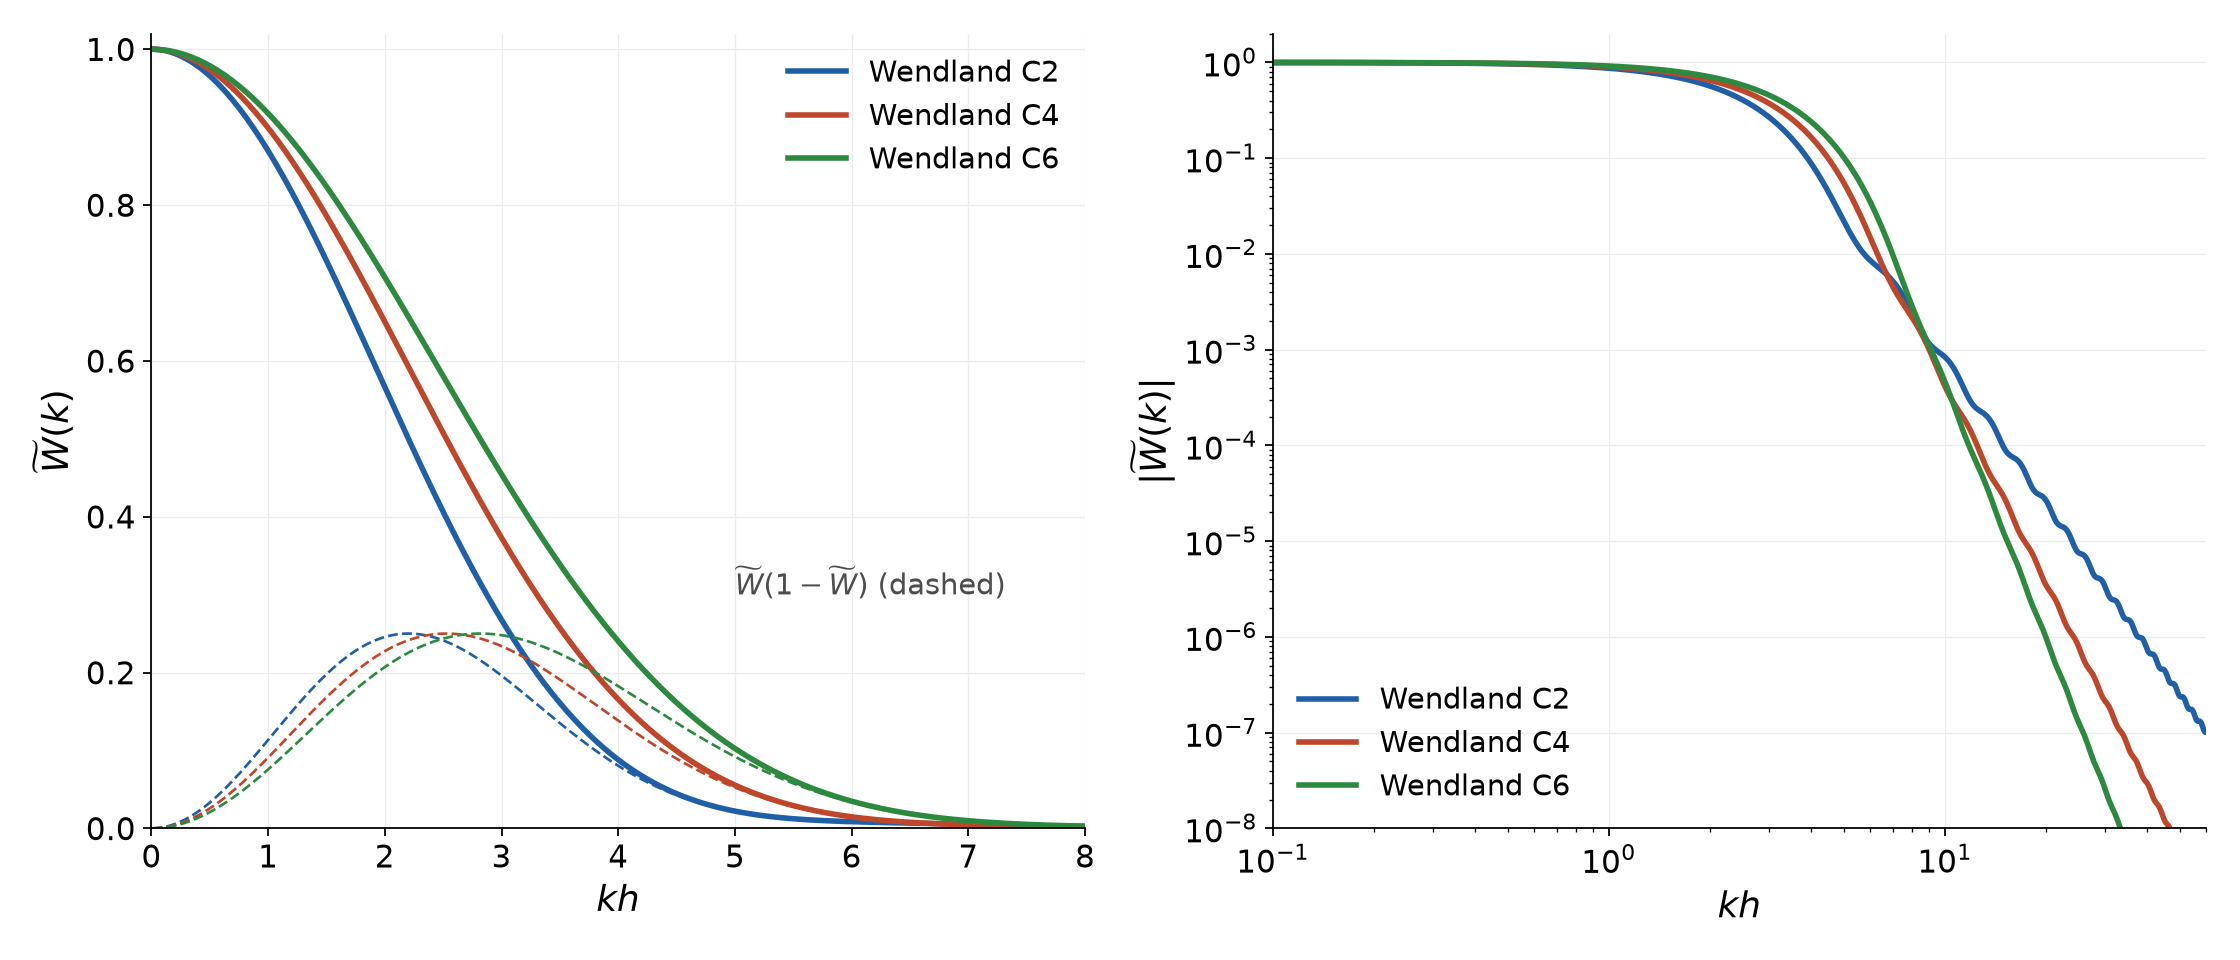
\includegraphics[width=0.6\textwidth]{figs/wendland_ft.png}
\caption{The Fourier transforms of the Wendland kernels.}
\label{fig:wft}
\end{figure}

\begin{thebibliography}{9}
\bibitem{amt} Y.~Akamatsu, A.~Mazeliauskas and D.~Teaney, \emph{Bulk viscosity from hydrodynamic fluctuations with relativistic hydro-kinetic theory},
  Phys.\ Rev.\ C \textbf{97}, 024902 (2018), arXiv:1708.05657.
\end{thebibliography}

\end{document}
